\chapter{Implementation}
\label{chap:implementation}

\section{Chosen Software Architecture}
In the given setting, the most accessible frontend is commonly a JavaScript web application.

To still make the classification run as quickly and efficiently as possible, a C++ binary runs in the backend providing an HTTP API to the frontend application.
In order to allow for more flexibility of the HTTP server, the initial approach was to pipe requests through a dedicated web application framework with database access that would allow, for instance, user management next to the basic classification.
However, the resulting communication and computation overhead, even when running with very efficient protocols such as ZeroMQ, was too high.

Extending the accessibility argument to reproducibility, Docker is a very solid choice \parencite{using-docker-in-science}.
To run the attached demo project, simply execute
\begin{minted}{bash}
  docker-compose build
  docker-compose up
\end{minted}
in the 'code' folder and point your browser to \url{https://localhost}.

\subsection{Docker Multi-Stage Build}
An enterprise-grade, scalable deployment is achieved by means of zero-dependency
Alpine Linux images which contain nothing but compiled binaries and linked libraries.

\section{The MNIST dataset}
The MNIST dataset \parencite{mnist-original} contains X train and Y test images with corresponding labels.
In order to stick to the traditional feedforward technique with data represented in vector format, therefore it is common to reshape data from $(28, 28)$ images (represented as grayscale values in a matrix)
into a $784$ element vector.

\section{Matrix-Vector Multiplication}
The dot product that is required as part of the neural network evaluation process needs to be implemented on SEAL ciphertexts as well.

There are multiple methods to achieve a syntactically correct dot product (matrix-vector multiplication) as described by \textcite{2018-gazelle} for (square) matrices.

\begin{enumerate}
  \item \textbf{Naïve MatMul} - very simple to derive but impractical in practice due to the limited further
        applicability of the result consisting of multiple ciphertexts. Applicable to arbitrary matrix dimensions,
        i.e. matrices $M \in \R^{s \times t}$, of course limited by the unreasonably high memory consumption
        and computation time of this approach.
  \item \textbf{Diagonal MatMul} - a simple and practical solution applicable to square matrices $M \in \R^{t \times t}$
        that has a major advantage compared to the previous method as the computation yields a
        single ciphertext object instead of many which can be directly passed on to a following evaluation operation.
  \item \textbf{Hybrid MatMul} - essentially extending the diagonal method by generalising the definition of the
        diagonal extraction mechanism to 'wrap around' in order to match the dimensionality of the input vector.
        Applicable to arbitrary matrix dimensions, i.e. matrices $M \in \R^{s \times t}$ and favourable compared
        to the Naïve Method.
  \item \textbf{Babystep-Giantstep MatMul} - a more sophisticated technique aiming to significantly reduce the number of
        Galois rotations as they are rather expensive to carry out,
        with a performance boost especially noticeable for higher matrix dimensions.
        Without further modification, applicable to square matrices.
\end{enumerate}

For the following, define
\newcommand{\rot}{\mathrm{rot}}
\newcommand{\diag}{\mathrm{diag}}
\begin{align}
  \rot_j: \R^t \mapsto \R^t,             & \; \{\rot_j(\vec{x})\}_i = x_{i + j} \label{eq:rot-definition} \\
  \diag_j: \R^{t \times t} \mapsto \R^t, & \; \{\diag_j(M)\}_i = M_{i, (i+j)} \label{eq:diag-definition}
\end{align}
with all indices $i, j \in \Z_t$ member of the cyclic quotient group $\Z_t := \Z / t \Z$ of all integers modulo $t$, meaning that overflowing indices simply wrap around again starting at index $0$ to simplify notation.
For the sake of compactness, we stick to this notation for the rest of this section.

\subsection{Adapting to non-square matrices}
\label{subsec:non-square-matrices}
The weight matrices in the given classification setting are by no means square, on the contrary their output dimension tends to be much lower than the input dimension as the goal is to reduce it from $28^2 = 784$ to $10$ overall.

However, that also means one cannot directly apply the diagonal method as described in the proceedings above.
This 'flaw' can be mitigated by a simple zero-padding approach in order to make the matrix square, filling in zeroes until the lower dimension reaches the higher one.

\subsection{The Naïve Method}
\begin{figure}[H]
  \centering
  \definecolor{c91d04f}{RGB}{145,208,79}
\definecolor{cdbe6f1}{RGB}{219,230,241}
\definecolor{cfefffe}{RGB}{254,255,254}
\definecolor{cf1dcda}{RGB}{241,220,218}
\definecolor{ce5b9b7}{RGB}{229,185,183}
\definecolor{cd89693}{RGB}{216,150,147}
\definecolor{cbf504c}{RGB}{191,80,76}
\definecolor{cb8cde4}{RGB}{184,205,228}
\definecolor{cbdbdbd}{RGB}{189,189,189}
\definecolor{cbebebe}{RGB}{190,190,190}
\definecolor{c94b3d6}{RGB}{148,179,214}
\definecolor{cd8d9d8}{RGB}{216,217,216}
\definecolor{cfeff00}{RGB}{254,255,0}
\definecolor{ccbc1d9}{RGB}{203,193,217}
\definecolor{c4f81bd}{RGB}{79,129,189}
\def \globalscale {12}
\newcommand{\naivematrix}{
  \begin{scope}[cm={{0.26458,0.0,0.0,0.26458,(30.6197,84.5995)}},even odd rule]
    \path[fill=black] (4.8948,11.5094) .. controls (13.3615,11.5094) and
    (21.8281,11.5094) .. (30.2948,11.5094) .. controls (30.2948,19.9760) and
    (30.2948,28.4427) .. (30.2948,36.9094) .. controls (21.8281,36.9094) and
    (13.3615,36.9094) .. (4.8948,36.9094) .. controls (4.8948,28.4427) and
    (4.8948,19.9760) .. (4.8948,11.5094) -- cycle;
    \path[fill=c91d04f] (5.4240,12.0385) .. controls (7.2760,12.0385) and
    (9.1281,12.0385) .. (10.9802,12.0385) .. controls (10.9802,13.8906) and
    (10.9802,15.7427) .. (10.9802,17.5948) .. controls (9.1281,17.5948) and
    (7.2760,17.5948) .. (5.4240,17.5948) .. controls (5.4240,15.7427) and
    (5.4240,13.8906) .. (5.4240,12.0385) -- cycle;
    \path[fill=c91d04f] (11.5094,12.0385) .. controls (13.4496,12.0385) and
    (15.3899,12.0385) .. (17.3302,12.0385) .. controls (17.3302,13.8906) and
    (17.3302,15.7427) .. (17.3302,17.5948) .. controls (15.3899,17.5948) and
    (13.4496,17.5948) .. (11.5094,17.5948) .. controls (11.5094,15.7427) and
    (11.5094,13.8906) .. (11.5094,12.0385) -- cycle;
    \path[fill=c91d04f] (17.8594,12.0385) .. controls (19.7996,12.0385) and
    (21.7399,12.0385) .. (23.6802,12.0385) .. controls (23.6802,13.8906) and
    (23.6802,15.7427) .. (23.6802,17.5948) .. controls (21.7399,17.5948) and
    (19.7996,17.5948) .. (17.8594,17.5948) .. controls (17.8594,15.7427) and
    (17.8594,13.8906) .. (17.8594,12.0385) -- cycle;
    \path[fill=c91d04f] (24.2094,12.0385) .. controls (26.0615,12.0385) and
    (27.9135,12.0385) .. (29.7656,12.0385) .. controls (29.7656,13.8906) and
    (29.7656,15.7427) .. (29.7656,17.5948) .. controls (27.9135,17.5948) and
    (26.0615,17.5948) .. (24.2094,17.5948) .. controls (24.2094,15.7427) and
    (24.2094,13.8906) .. (24.2094,12.0385) -- cycle;
    \path[fill=cfeff00] (5.4240,18.1240) .. controls (7.2760,18.1240) and
    (9.1281,18.1240) .. (10.9802,18.1240) .. controls (10.9802,20.0642) and
    (10.9802,22.0045) .. (10.9802,23.9448) .. controls (9.1281,23.9448) and
    (7.2760,23.9448) .. (5.4240,23.9448) .. controls (5.4240,22.0045) and
    (5.4240,20.0642) .. (5.4240,18.1240) -- cycle;
    \path[fill=cfeff00] (11.5094,18.1240) .. controls (13.4496,18.1240) and
    (15.3899,18.1240) .. (17.3302,18.1240) .. controls (17.3302,20.0642) and
    (17.3302,22.0045) .. (17.3302,23.9448) .. controls (15.3899,23.9448) and
    (13.4496,23.9448) .. (11.5094,23.9448) .. controls (11.5094,22.0045) and
    (11.5094,20.0642) .. (11.5094,18.1240) -- cycle;
    \path[fill=cfeff00] (17.8594,18.1240) .. controls (19.7996,18.1240) and
    (21.7399,18.1240) .. (23.6802,18.1240) .. controls (23.6802,20.0642) and
    (23.6802,22.0045) .. (23.6802,23.9448) .. controls (21.7399,23.9448) and
    (19.7996,23.9448) .. (17.8594,23.9448) .. controls (17.8594,22.0045) and
    (17.8594,20.0642) .. (17.8594,18.1240) -- cycle;
    \path[fill=cfeff00] (24.2094,18.1240) .. controls (26.0615,18.1240) and
    (27.9135,18.1240) .. (29.7656,18.1240) .. controls (29.7656,20.0642) and
    (29.7656,22.0045) .. (29.7656,23.9448) .. controls (27.9135,23.9448) and
    (26.0615,23.9448) .. (24.2094,23.9448) .. controls (24.2094,22.0045) and
    (24.2094,20.0642) .. (24.2094,18.1240) -- cycle;
    \path[fill=ccbc1d9] (5.4240,24.4740) .. controls (7.2760,24.4740) and
    (9.1281,24.4740) .. (10.9802,24.4740) .. controls (10.9802,26.3260) and
    (10.9802,28.1781) .. (10.9802,30.0302) .. controls (9.1281,30.0302) and
    (7.2760,30.0302) .. (5.4240,30.0302) .. controls (5.4240,28.1781) and
    (5.4240,26.3260) .. (5.4240,24.4740) -- cycle;
    \path[fill=ccbc1d9] (11.5094,24.4740) .. controls (13.4496,24.4740) and
    (15.3899,24.4740) .. (17.3302,24.4740) .. controls (17.3302,26.3260) and
    (17.3302,28.1781) .. (17.3302,30.0302) .. controls (15.3899,30.0302) and
    (13.4496,30.0302) .. (11.5094,30.0302) .. controls (11.5094,28.1781) and
    (11.5094,26.3260) .. (11.5094,24.4740) -- cycle;
    \path[fill=ccbc1d9] (17.8594,24.4740) .. controls (19.7996,24.4740) and
    (21.7399,24.4740) .. (23.6802,24.4740) .. controls (23.6802,26.3260) and
    (23.6802,28.1781) .. (23.6802,30.0302) .. controls (21.7399,30.0302) and
    (19.7996,30.0302) .. (17.8594,30.0302) .. controls (17.8594,28.1781) and
    (17.8594,26.3260) .. (17.8594,24.4740) -- cycle;
    \path[fill=ccbc1d9] (24.2094,24.4740) .. controls (26.0615,24.4740) and
    (27.9135,24.4740) .. (29.7656,24.4740) .. controls (29.7656,26.3260) and
    (29.7656,28.1781) .. (29.7656,30.0302) .. controls (27.9135,30.0302) and
    (26.0615,30.0302) .. (24.2094,30.0302) .. controls (24.2094,28.1781) and
    (24.2094,26.3260) .. (24.2094,24.4740) -- cycle;
    \path[fill=cd8d9d8] (5.4240,30.5594) .. controls (7.2760,30.5594) and
    (9.1281,30.5594) .. (10.9802,30.5594) .. controls (10.9802,32.4996) and
    (10.9802,34.4400) .. (10.9802,36.3802) .. controls (9.1281,36.3802) and
    (7.2760,36.3802) .. (5.4240,36.3802) .. controls (5.4240,34.4400) and
    (5.4240,32.4996) .. (5.4240,30.5594) -- cycle;
    \path[fill=cd8d9d8] (11.5094,30.5594) .. controls (13.4496,30.5594) and
    (15.3899,30.5594) .. (17.3302,30.5594) .. controls (17.3302,32.4996) and
    (17.3302,34.4400) .. (17.3302,36.3802) .. controls (15.3899,36.3802) and
    (13.4496,36.3802) .. (11.5094,36.3802) .. controls (11.5094,34.4400) and
    (11.5094,32.4996) .. (11.5094,30.5594) -- cycle;
    \path[fill=cd8d9d8] (17.8594,30.5594) .. controls (19.7996,30.5594) and
    (21.7399,30.5594) .. (23.6802,30.5594) .. controls (23.6802,32.4996) and
    (23.6802,34.4400) .. (23.6802,36.3802) .. controls (21.7399,36.3802) and
    (19.7996,36.3802) .. (17.8594,36.3802) .. controls (17.8594,34.4400) and
    (17.8594,32.4996) .. (17.8594,30.5594) -- cycle;
    \path[fill=cd8d9d8] (24.2094,30.5594) .. controls (26.0615,30.5594) and
    (27.9135,30.5594) .. (29.7656,30.5594) .. controls (29.7656,32.4996) and
    (29.7656,34.4400) .. (29.7656,36.3802) .. controls (27.9135,36.3802) and
    (26.0615,36.3802) .. (24.2094,36.3802) .. controls (24.2094,34.4400) and
    (24.2094,32.4996) .. (24.2094,30.5594) -- cycle;
  \end{scope}
}

\begin{tikzpicture}[y=0.80pt, x=0.80pt, yscale=-\globalscale, xscale=\globalscale, inner sep=0pt, outer sep=0pt]
  \begin{scope}
    \draw (5.7,6)    node {\Large $\times$};
    \draw (10.8,6)   node {\Large $\Rightarrow$};
    \draw (16.2,2.3) node {$\times$};
    \draw (16.2,5.9) node {\Large $+ \ldots +$};
    \draw (16.2,9.6) node {$\times$};
    \draw (21.8,6)   node {\Large $\Rightarrow$};
  \end{scope}
  \begin{scope}[shift={(-34.3145,-85.1193)}]
    \naivematrix
    \begin{scope}[cm={{0.26458,0.0,0.0,0.26458,(30.6197,84.5995)}},even odd rule]
      \path[fill=black] (62.8385,1.7198) .. controls (71.3052,1.7198) and
      (79.7719,1.7198) .. (88.2385,1.7198) .. controls (88.2385,4.0129) and
      (88.2385,6.3059) .. (88.2385,8.5990) .. controls (79.7719,8.5990) and
      (71.3052,8.5990) .. (62.8385,8.5990) .. controls (62.8385,6.3059) and
      (62.8385,4.0129) .. (62.8385,1.7198) -- cycle;
      \path[fill=c91d04f] (63.3677,2.2490) .. controls (65.2198,2.2490) and
      (67.0719,2.2490) .. (68.9240,2.2490) .. controls (68.9240,4.1892) and
      (68.9240,6.1295) .. (68.9240,8.0698) .. controls (67.0719,8.0698) and
      (65.2198,8.0698) .. (63.3677,8.0698) .. controls (63.3677,6.1295) and
      (63.3677,4.1892) .. (63.3677,2.2490) -- cycle;
      \path[fill=c91d04f] (69.4531,2.2490) .. controls (71.3933,2.2490) and
      (73.3338,2.2490) .. (75.2740,2.2490) .. controls (75.2740,4.1892) and
      (75.2740,6.1295) .. (75.2740,8.0698) .. controls (73.3338,8.0698) and
      (71.3933,8.0698) .. (69.4531,8.0698) .. controls (69.4531,6.1295) and
      (69.4531,4.1892) .. (69.4531,2.2490) -- cycle;
      \path[fill=c91d04f] (75.8031,2.2490) .. controls (77.6552,2.2490) and
      (79.5073,2.2490) .. (81.3594,2.2490) .. controls (81.3594,4.1892) and
      (81.3594,6.1295) .. (81.3594,8.0698) .. controls (79.5073,8.0698) and
      (77.6552,8.0698) .. (75.8031,8.0698) .. controls (75.8031,6.1295) and
      (75.8031,4.1892) .. (75.8031,2.2490) -- cycle;
      \path[fill=c91d04f] (81.8885,2.2490) .. controls (83.8287,2.2490) and
      (85.7692,2.2490) .. (87.7094,2.2490) .. controls (87.7094,4.1892) and
      (87.7094,6.1295) .. (87.7094,8.0698) .. controls (85.7692,8.0698) and
      (83.8287,8.0698) .. (81.8885,8.0698) .. controls (81.8885,6.1295) and
      (81.8885,4.1892) .. (81.8885,2.2490) -- cycle;
    \end{scope}
    \begin{scope}[cm={{0.26458,0.0,0.0,0.26458,(30.6197,84.5995)}},even odd rule]
      \path[fill=black] (104.3781,9.6573) .. controls (112.9329,9.6573) and
      (121.4879,9.6573) .. (130.0427,9.6573) .. controls (130.0427,11.9504) and
      (130.0427,14.2434) .. (130.0427,16.5365) .. controls (121.4879,16.5365) and
      (112.9329,16.5365) .. (104.3781,16.5365) .. controls (104.3781,14.2434) and
      (104.3781,11.9504) .. (104.3781,9.6573) -- cycle;
    \end{scope}
    \begin{scope}[cm={{0.26458,0.0,0.0,0.26458,(30.6197,84.5995)}},even odd rule]
      \path[fill=cdbe6f1] (104.9073,10.1865) .. controls (106.8475,10.1865) and
      (108.7879,10.1865) .. (110.7281,10.1865) .. controls (110.7281,12.1267) and
      (110.7281,14.0670) .. (110.7281,16.0073) .. controls (108.7879,16.0073) and
      (106.8475,16.0073) .. (104.9073,16.0073) .. controls (104.9073,14.0670) and
      (104.9073,12.1267) .. (104.9073,10.1865) -- cycle;
    \end{scope}
    \begin{scope}[cm={{0.26458,0.0,0.0,0.26458,(30.6197,84.5995)}},even odd rule]
      \path[fill=cfefffe] (111.2573,10.1865) .. controls (113.1975,10.1865) and
      (115.1379,10.1865) .. (117.0781,10.1865) .. controls (117.0781,12.1267) and
      (117.0781,14.0670) .. (117.0781,16.0073) .. controls (115.1379,16.0073) and
      (113.1975,16.0073) .. (111.2573,16.0073) .. controls (111.2573,14.0670) and
      (111.2573,12.1267) .. (111.2573,10.1865) -- cycle;
    \end{scope}
    \begin{scope}[cm={{0.26458,0.0,0.0,0.26458,(30.6197,84.5995)}},even odd rule]
      \path[fill=cfefffe] (117.6073,10.1865) .. controls (119.4594,10.1865) and
      (121.3115,10.1865) .. (123.1635,10.1865) .. controls (123.1635,12.1267) and
      (123.1635,14.0670) .. (123.1635,16.0073) .. controls (121.3115,16.0073) and
      (119.4594,16.0073) .. (117.6073,16.0073) .. controls (117.6073,14.0670) and
      (117.6073,12.1267) .. (117.6073,10.1865) -- cycle;
    \end{scope}
    \begin{scope}[cm={{0.26458,0.0,0.0,0.26458,(30.6197,84.5995)}},even odd rule]
      \path[fill=cfefffe] (123.6927,10.1865) .. controls (125.6329,10.1865) and
      (127.5734,10.1865) .. (129.5135,10.1865) .. controls (129.5135,12.1267) and
      (129.5135,14.0670) .. (129.5135,16.0073) .. controls (127.5734,16.0073) and
      (125.6329,16.0073) .. (123.6927,16.0073) .. controls (123.6927,14.0670) and
      (123.6927,12.1267) .. (123.6927,10.1865) -- cycle;
    \end{scope}
    \begin{scope}[cm={{0.26458,0.0,0.0,0.26458,(30.6197,84.5995)}},even odd rule]
      \path[fill=black] (62.8385,12.8323) .. controls (71.3052,12.8323) and
      (79.7719,12.8323) .. (88.2385,12.8323) .. controls (88.2385,15.1254) and
      (88.2385,17.4184) .. (88.2385,19.7115) .. controls (79.7719,19.7115) and
      (71.3052,19.7115) .. (62.8385,19.7115) .. controls (62.8385,17.4184) and
      (62.8385,15.1254) .. (62.8385,12.8323) -- cycle;
    \end{scope}
    \begin{scope}[cm={{0.26458,0.0,0.0,0.26458,(30.6197,84.5995)}},even odd rule]
      \path[fill=cf1dcda] (63.3677,13.3615) .. controls (65.2198,13.3615) and
      (67.0719,13.3615) .. (68.9240,13.3615) .. controls (68.9240,15.3017) and
      (68.9240,17.2420) .. (68.9240,19.1823) .. controls (67.0719,19.1823) and
      (65.2198,19.1823) .. (63.3677,19.1823) .. controls (63.3677,17.2420) and
      (63.3677,15.3017) .. (63.3677,13.3615) -- cycle;
    \end{scope}
    \begin{scope}[cm={{0.26458,0.0,0.0,0.26458,(30.6197,84.5995)}},even odd rule]
      \path[fill=ce5b9b7] (69.4531,13.3615) .. controls (71.3933,13.3615) and
      (73.3338,13.3615) .. (75.2740,13.3615) .. controls (75.2740,15.3017) and
      (75.2740,17.2420) .. (75.2740,19.1823) .. controls (73.3338,19.1823) and
      (71.3933,19.1823) .. (69.4531,19.1823) .. controls (69.4531,17.2420) and
      (69.4531,15.3017) .. (69.4531,13.3615) -- cycle;
    \end{scope}
    \begin{scope}[cm={{0.26458,0.0,0.0,0.26458,(30.6197,84.5995)}},even odd rule]
      \path[fill=cd89693] (75.8031,13.3615) .. controls (77.6552,13.3615) and
      (79.5073,13.3615) .. (81.3594,13.3615) .. controls (81.3594,15.3017) and
      (81.3594,17.2420) .. (81.3594,19.1823) .. controls (79.5073,19.1823) and
      (77.6552,19.1823) .. (75.8031,19.1823) .. controls (75.8031,17.2420) and
      (75.8031,15.3017) .. (75.8031,13.3615) -- cycle;
    \end{scope}
    \begin{scope}[cm={{0.26458,0.0,0.0,0.26458,(30.6197,84.5995)}},even odd rule]
      \path[fill=cbf504c] (81.8885,13.3615) .. controls (83.8287,13.3615) and
      (85.7692,13.3615) .. (87.7094,13.3615) .. controls (87.7094,15.3017) and
      (87.7094,17.2420) .. (87.7094,19.1823) .. controls (85.7692,19.1823) and
      (83.8287,19.1823) .. (81.8885,19.1823) .. controls (81.8885,17.2420) and
      (81.8885,15.3017) .. (81.8885,13.3615) -- cycle;
    \end{scope}
    \begin{scope}[cm={{0.26458,0.0,0.0,0.26458,(30.6197,84.5995)}},even odd rule]
      \path[fill=black] (104.3781,17.3302) .. controls (112.9329,17.3302) and
      (121.4879,17.3302) .. (130.0427,17.3302) .. controls (130.0427,19.6233) and
      (130.0427,21.9163) .. (130.0427,24.2094) .. controls (121.4879,24.2094) and
      (112.9329,24.2094) .. (104.3781,24.2094) .. controls (104.3781,21.9163) and
      (104.3781,19.6233) .. (104.3781,17.3302) -- cycle;
    \end{scope}
    \begin{scope}[cm={{0.26458,0.0,0.0,0.26458,(30.6197,84.5995)}},even odd rule]
      \path[fill=cb8cde4] (104.9073,17.8594) .. controls (106.8475,17.8594) and
      (108.7879,17.8594) .. (110.7281,17.8594) .. controls (110.7281,19.7996) and
      (110.7281,21.7399) .. (110.7281,23.6802) .. controls (108.7879,23.6802) and
      (106.8475,23.6802) .. (104.9073,23.6802) .. controls (104.9073,21.7399) and
      (104.9073,19.7996) .. (104.9073,17.8594) -- cycle;
    \end{scope}
    \begin{scope}[cm={{0.26458,0.0,0.0,0.26458,(30.6197,84.5995)}},even odd rule]
      \path[fill=cfefffe] (111.2573,17.8594) .. controls (113.1975,17.8594) and
      (115.1379,17.8594) .. (117.0781,17.8594) .. controls (117.0781,19.7996) and
      (117.0781,21.7399) .. (117.0781,23.6802) .. controls (115.1379,23.6802) and
      (113.1975,23.6802) .. (111.2573,23.6802) .. controls (111.2573,21.7399) and
      (111.2573,19.7996) .. (111.2573,17.8594) -- cycle;
    \end{scope}
    \begin{scope}[cm={{0.26458,0.0,0.0,0.26458,(30.6197,84.5995)}},even odd rule]
      \path[fill=cfefffe] (117.6073,17.8594) .. controls (119.4594,17.8594) and
      (121.3115,17.8594) .. (123.1635,17.8594) .. controls (123.1635,19.7996) and
      (123.1635,21.7399) .. (123.1635,23.6802) .. controls (121.3115,23.6802) and
      (119.4594,23.6802) .. (117.6073,23.6802) .. controls (117.6073,21.7399) and
      (117.6073,19.7996) .. (117.6073,17.8594) -- cycle;
    \end{scope}
    \begin{scope}[cm={{0.26458,0.0,0.0,0.26458,(30.6197,84.5995)}},even odd rule]
      \path[fill=cfefffe] (123.6927,17.8594) .. controls (125.6329,17.8594) and
      (127.5734,17.8594) .. (129.5135,17.8594) .. controls (129.5135,19.7996) and
      (129.5135,21.7399) .. (129.5135,23.6802) .. controls (127.5734,23.6802) and
      (125.6329,23.6802) .. (123.6927,23.6802) .. controls (123.6927,21.7399) and
      (123.6927,19.7996) .. (123.6927,17.8594) -- cycle;
    \end{scope}
    \begin{scope}[cm={{0.26458,0.0,0.0,0.26458,(30.6197,84.5995)}},even odd rule]
      \path[fill=black] (130.3073,25.0031) .. controls (130.3073,27.2079) and
      (130.3073,29.4129) .. (130.3073,31.6177) .. controls (121.7525,31.6177) and
      (113.1975,31.6177) .. (104.6427,31.6177) .. controls (104.6427,29.4129) and
      (104.6427,27.2079) .. (104.6427,25.0031) .. controls (113.1975,25.0031) and
      (121.7525,25.0031) .. (130.3073,25.0031) -- cycle;
    \end{scope}
    \begin{scope}[cm={{0.26458,0.0,0.0,0.26458,(30.6197,84.5995)}},even odd rule]
      \path[fill=c94b3d6] (105.1719,25.5323) .. controls (107.1121,25.5323) and
      (109.0525,25.5323) .. (110.9927,25.5323) .. controls (110.9927,27.3844) and
      (110.9927,29.2365) .. (110.9927,31.0885) .. controls (109.0525,31.0885) and
      (107.1121,31.0885) .. (105.1719,31.0885) .. controls (105.1719,29.2365) and
      (105.1719,27.3844) .. (105.1719,25.5323) -- cycle;
    \end{scope}
    \begin{scope}[cm={{0.26458,0.0,0.0,0.26458,(30.6197,84.5995)}},even odd rule]
      \path[fill=cfefffe] (111.5219,25.5323) .. controls (113.3740,25.5323) and
      (115.2260,25.5323) .. (117.0781,25.5323) .. controls (117.0781,27.3844) and
      (117.0781,29.2365) .. (117.0781,31.0885) .. controls (115.2260,31.0885) and
      (113.3740,31.0885) .. (111.5219,31.0885) .. controls (111.5219,29.2365) and
      (111.5219,27.3844) .. (111.5219,25.5323) -- cycle;
    \end{scope}
    \begin{scope}[cm={{0.26458,0.0,0.0,0.26458,(30.6197,84.5995)}},even odd rule]
      \path[fill=cfefffe] (117.6073,25.5323) .. controls (119.5475,25.5323) and
      (121.4879,25.5323) .. (123.4281,25.5323) .. controls (123.4281,27.3844) and
      (123.4281,29.2365) .. (123.4281,31.0885) .. controls (121.4879,31.0885) and
      (119.5475,31.0885) .. (117.6073,31.0885) .. controls (117.6073,29.2365) and
      (117.6073,27.3844) .. (117.6073,25.5323) -- cycle;
    \end{scope}
    \begin{scope}[cm={{0.26458,0.0,0.0,0.26458,(30.6197,84.5995)}},even odd rule]
      \path[fill=cfefffe] (123.9573,25.5323) .. controls (125.8975,25.5323) and
      (127.8379,25.5323) .. (129.7781,25.5323) .. controls (129.7781,27.3844) and
      (129.7781,29.2365) .. (129.7781,31.0885) .. controls (127.8379,31.0885) and
      (125.8975,31.0885) .. (123.9573,31.0885) .. controls (123.9573,29.2365) and
      (123.9573,27.3844) .. (123.9573,25.5323) -- cycle;
    \end{scope}
    \begin{scope}[cm={{0.26458,0.0,0.0,0.26458,(30.6197,84.5995)}},even odd rule]
      \path[fill=black] (62.8385,29.2365) .. controls (71.3052,29.2365) and
      (79.7719,29.2365) .. (88.2385,29.2365) .. controls (88.2385,31.5296) and
      (88.2385,33.8225) .. (88.2385,36.1156) .. controls (79.7719,36.1156) and
      (71.3052,36.1156) .. (62.8385,36.1156) .. controls (62.8385,33.8225) and
      (62.8385,31.5296) .. (62.8385,29.2365) -- cycle;
    \end{scope}
    \begin{scope}[cm={{0.26458,0.0,0.0,0.26458,(30.6197,84.5995)}},even odd rule]
      \path[fill=cd8d9d8] (63.3677,29.7656) .. controls (65.2198,29.7656) and
      (67.0719,29.7656) .. (68.9240,29.7656) .. controls (68.9240,31.7058) and
      (68.9240,33.6463) .. (68.9240,35.5865) .. controls (67.0719,35.5865) and
      (65.2198,35.5865) .. (63.3677,35.5865) .. controls (63.3677,33.6463) and
      (63.3677,31.7058) .. (63.3677,29.7656) -- cycle;
    \end{scope}
    \begin{scope}[cm={{0.26458,0.0,0.0,0.26458,(30.6197,84.5995)}},even odd rule]
      \path[fill=cd8d9d8] (69.4531,29.7656) .. controls (71.3933,29.7656) and
      (73.3338,29.7656) .. (75.2740,29.7656) .. controls (75.2740,31.7058) and
      (75.2740,33.6463) .. (75.2740,35.5865) .. controls (73.3338,35.5865) and
      (71.3933,35.5865) .. (69.4531,35.5865) .. controls (69.4531,33.6463) and
      (69.4531,31.7058) .. (69.4531,29.7656) -- cycle;
    \end{scope}
    \begin{scope}[cm={{0.26458,0.0,0.0,0.26458,(30.6197,84.5995)}},even odd rule]
      \path[fill=cd8d9d8] (75.8031,29.7656) .. controls (77.6552,29.7656) and
      (79.5073,29.7656) .. (81.3594,29.7656) .. controls (81.3594,31.7058) and
      (81.3594,33.6463) .. (81.3594,35.5865) .. controls (79.5073,35.5865) and
      (77.6552,35.5865) .. (75.8031,35.5865) .. controls (75.8031,33.6463) and
      (75.8031,31.7058) .. (75.8031,29.7656) -- cycle;
    \end{scope}
    \begin{scope}[cm={{0.26458,0.0,0.0,0.26458,(30.6197,84.5995)}},even odd rule]
      \path[fill=cd8d9d8] (81.8885,29.7656) .. controls (83.8287,29.7656) and
      (85.7692,29.7656) .. (87.7094,29.7656) .. controls (87.7094,31.7058) and
      (87.7094,33.6463) .. (87.7094,35.5865) .. controls (85.7692,35.5865) and
      (83.8287,35.5865) .. (81.8885,35.5865) .. controls (81.8885,33.6463) and
      (81.8885,31.7058) .. (81.8885,29.7656) -- cycle;
    \end{scope}
    \begin{scope}[cm={{0.26458,0.0,0.0,0.26458,(30.6197,84.5995)}},even odd rule]
      \path[fill=black] (40.3490,11.5094) .. controls (42.5537,11.5094) and
      (44.7588,11.5094) .. (46.9635,11.5094) .. controls (46.9635,19.9760) and
      (46.9635,28.4427) .. (46.9635,36.9094) .. controls (44.7588,36.9094) and
      (42.5537,36.9094) .. (40.3490,36.9094) .. controls (40.3490,28.4427) and
      (40.3490,19.9760) .. (40.3490,11.5094) -- cycle;
      \path[fill=cf1dcda] (40.8781,12.0385) .. controls (42.7302,12.0385) and
      (44.5823,12.0385) .. (46.4344,12.0385) .. controls (46.4344,13.8906) and
      (46.4344,15.7427) .. (46.4344,17.5948) .. controls (44.5823,17.5948) and
      (42.7302,17.5948) .. (40.8781,17.5948) .. controls (40.8781,15.7427) and
      (40.8781,13.8906) .. (40.8781,12.0385) -- cycle;
      \path[fill=ce5b9b7] (40.8781,18.1240) .. controls (42.7302,18.1240) and
      (44.5823,18.1240) .. (46.4344,18.1240) .. controls (46.4344,20.0642) and
      (46.4344,22.0045) .. (46.4344,23.9448) .. controls (44.5823,23.9448) and
      (42.7302,23.9448) .. (40.8781,23.9448) .. controls (40.8781,22.0045) and
      (40.8781,20.0642) .. (40.8781,18.1240) -- cycle;
      \path[fill=cd89693] (40.8781,24.4740) .. controls (42.7302,24.4740) and
      (44.5823,24.4740) .. (46.4344,24.4740) .. controls (46.4344,26.3260) and
      (46.4344,28.1781) .. (46.4344,30.0302) .. controls (44.5823,30.0302) and
      (42.7302,30.0302) .. (40.8781,30.0302) .. controls (40.8781,28.1781) and
      (40.8781,26.3260) .. (40.8781,24.4740) -- cycle;
      \path[fill=cbf504c] (40.8781,30.5594) .. controls (42.7302,30.5594) and
      (44.5823,30.5594) .. (46.4344,30.5594) .. controls (46.4344,32.4996) and
      (46.4344,34.4400) .. (46.4344,36.3802) .. controls (44.5823,36.3802) and
      (42.7302,36.3802) .. (40.8781,36.3802) .. controls (40.8781,34.4400) and
      (40.8781,32.4996) .. (40.8781,30.5594) -- cycle;
    \end{scope}
    \begin{scope}[cm={{0.26458,0.0,0.0,0.26458,(30.6197,84.5995)}},even odd rule]
      \path[fill=black] (130.3073,32.6760) .. controls (130.3073,34.8808) and
      (130.3073,37.0859) .. (130.3073,39.2906) .. controls (121.7525,39.2906) and
      (113.1975,39.2906) .. (104.6427,39.2906) .. controls (104.6427,37.0859) and
      (104.6427,34.8808) .. (104.6427,32.6760) .. controls (113.1975,32.6760) and
      (121.7525,32.6760) .. (130.3073,32.6760) -- cycle;
    \end{scope}
    \begin{scope}[cm={{0.26458,0.0,0.0,0.26458,(30.6197,84.5995)}},even odd rule]
      \path[fill=c4f81bd] (105.1719,33.2052) .. controls (107.1121,33.2052) and
      (109.0525,33.2052) .. (110.9927,33.2052) .. controls (110.9927,35.0573) and
      (110.9927,36.9094) .. (110.9927,38.7615) .. controls (109.0525,38.7615) and
      (107.1121,38.7615) .. (105.1719,38.7615) .. controls (105.1719,36.9094) and
      (105.1719,35.0573) .. (105.1719,33.2052) -- cycle;
    \end{scope}
    \begin{scope}[cm={{0.26458,0.0,0.0,0.26458,(30.6197,84.5995)}},even odd rule]
      \path[fill=cfefffe] (111.5219,33.2052) .. controls (113.3740,33.2052) and
      (115.2260,33.2052) .. (117.0781,33.2052) .. controls (117.0781,35.0573) and
      (117.0781,36.9094) .. (117.0781,38.7615) .. controls (115.2260,38.7615) and
      (113.3740,38.7615) .. (111.5219,38.7615) .. controls (111.5219,36.9094) and
      (111.5219,35.0573) .. (111.5219,33.2052) -- cycle;
    \end{scope}
    \begin{scope}[cm={{0.26458,0.0,0.0,0.26458,(30.6197,84.5995)}},even odd rule]
      \path[fill=cfefffe] (117.6073,33.2052) .. controls (119.5475,33.2052) and
      (121.4879,33.2052) .. (123.4281,33.2052) .. controls (123.4281,35.0573) and
      (123.4281,36.9094) .. (123.4281,38.7615) .. controls (121.4879,38.7615) and
      (119.5475,38.7615) .. (117.6073,38.7615) .. controls (117.6073,36.9094) and
      (117.6073,35.0573) .. (117.6073,33.2052) -- cycle;
    \end{scope}
    \begin{scope}[cm={{0.26458,0.0,0.0,0.26458,(30.6197,84.5995)}},even odd rule]
      \path[fill=cfefffe] (123.9573,33.2052) .. controls (125.8975,33.2052) and
      (127.8379,33.2052) .. (129.7781,33.2052) .. controls (129.7781,35.0573) and
      (129.7781,36.9094) .. (129.7781,38.7615) .. controls (127.8379,38.7615) and
      (125.8975,38.7615) .. (123.9573,38.7615) .. controls (123.9573,36.9094) and
      (123.9573,35.0573) .. (123.9573,33.2052) -- cycle;
    \end{scope}
    \begin{scope}[cm={{0.26458,0.0,0.0,0.26458,(30.6197,84.5995)}},even odd rule]
      \path[fill=black] (62.8385,40.3490) .. controls (71.3052,40.3490) and
      (79.7719,40.3490) .. (88.2385,40.3490) .. controls (88.2385,42.6421) and
      (88.2385,44.9350) .. (88.2385,47.2281) .. controls (79.7719,47.2281) and
      (71.3052,47.2281) .. (62.8385,47.2281) .. controls (62.8385,44.9350) and
      (62.8385,42.6421) .. (62.8385,40.3490) -- cycle;
    \end{scope}
    \begin{scope}[cm={{0.26458,0.0,0.0,0.26458,(30.6197,84.5995)}},even odd rule]
      \path[fill=cf1dcda] (63.3677,40.8781) .. controls (65.2198,40.8781) and
      (67.0719,40.8781) .. (68.9240,40.8781) .. controls (68.9240,42.8183) and
      (68.9240,44.7588) .. (68.9240,46.6990) .. controls (67.0719,46.6990) and
      (65.2198,46.6990) .. (63.3677,46.6990) .. controls (63.3677,44.7588) and
      (63.3677,42.8183) .. (63.3677,40.8781) -- cycle;
    \end{scope}
    \begin{scope}[cm={{0.26458,0.0,0.0,0.26458,(30.6197,84.5995)}},even odd rule]
      \path[fill=ce5b9b7] (69.4531,40.8781) .. controls (71.3933,40.8781) and
      (73.3338,40.8781) .. (75.2740,40.8781) .. controls (75.2740,42.8183) and
      (75.2740,44.7588) .. (75.2740,46.6990) .. controls (73.3338,46.6990) and
      (71.3933,46.6990) .. (69.4531,46.6990) .. controls (69.4531,44.7588) and
      (69.4531,42.8183) .. (69.4531,40.8781) -- cycle;
    \end{scope}
    \begin{scope}[cm={{0.26458,0.0,0.0,0.26458,(30.6197,84.5995)}},even odd rule]
      \path[fill=cd89693] (75.8031,40.8781) .. controls (77.6552,40.8781) and
      (79.5073,40.8781) .. (81.3594,40.8781) .. controls (81.3594,42.8183) and
      (81.3594,44.7588) .. (81.3594,46.6990) .. controls (79.5073,46.6990) and
      (77.6552,46.6990) .. (75.8031,46.6990) .. controls (75.8031,44.7588) and
      (75.8031,42.8183) .. (75.8031,40.8781) -- cycle;
    \end{scope}
    \begin{scope}[cm={{0.26458,0.0,0.0,0.26458,(30.6197,84.5995)}},even odd rule]
      \path[fill=cbf504c] (81.8885,40.8781) .. controls (83.8287,40.8781) and
      (85.7692,40.8781) .. (87.7094,40.8781) .. controls (87.7094,42.8183) and
      (87.7094,44.7588) .. (87.7094,46.6990) .. controls (85.7692,46.6990) and
      (83.8287,46.6990) .. (81.8885,46.6990) .. controls (81.8885,44.7588) and
      (81.8885,42.8183) .. (81.8885,40.8781) -- cycle;
    \end{scope}
  \end{scope}
\end{tikzpicture}

  \caption[Image adapted from \cite{2018-gazelle}]{The naïve method to multiply a square matrix with a vector.}
\end{figure}

Term by term, one can express a matrix-vector product of $M \in \R^{s \times t}$ and
$\vec{x} \in \R^s$ as follows:
$$\{M \vec{x}\}_i = \sum_{j=1}^{t} M_{ij} x_j$$

Accordingly, a natural (or rather, naïve) way to model this multiplication in \textit{Microsoft SEAL} would be to
\begin{enumerate}
  \item encode each $i$-th matrix row $(M_{i,1}, M_{i,2}, ..., M_{i,t})$ using the \cpp{Encoder}
        with matching parameters to the ciphertext of the encoded vector $\vec{x}$.
  \item multiply each encoded row with the encrypted vector using \cpp{Evaluator.multiply_plain()}
        to obtain the ciphertext vector $\vec{y_i} \in \R^s$ for row $i$.
  \item perform the 'rotate-and-sum' algorithm \parencite{2018-gazelle} on each
        resulting vector (ciphertext) $\vec{y_i}$ to obtain the actual dot product
        of the matrix row with the vector $\vec{x}$:
        \begin{enumerate}
          \item using Galois automorphisms, rotate the entries of $\vec{y_i}$ by $\frac{s}{2}$ elements
                to obtain $\rot_{\frac{s}{2}}(\vec{y_i})$.
          \item perform an element-wise sum $\vec{y_i} + \rot_{\frac{s}{2}}(\vec{y_i})$
                whose first (and also second) half now contains the sum of the two halves of $\vec{y_i}$.
          \item repeat the previous two steps $\log_2(s)$ times, halving the
                split parameter $s$ each time until one obtains $1$ element,
                which yields us the requested sum of all entries $\sum_{k=1}^s \{\vec{y_i}\}_k$
                as the dot product of $\vec{x}$ and $\vec{y_i}$.
        \end{enumerate}
  \item Given all the 'scalar' results of each row-vector dot product,
        we can construct the resulting matrix-vector product.
\end{enumerate}

\subsection{The Diagonal Method}
\begin{figure}[H]
  \centering
  \definecolor{c91d04f}{RGB}{145,208,79}
\definecolor{cf1dcda}{RGB}{241,220,218}
\definecolor{ce5b9b7}{RGB}{229,185,183}
\definecolor{cd89693}{RGB}{216,150,147}
\definecolor{cbf504c}{RGB}{191,80,76}
\definecolor{cfeff00}{RGB}{254,255,0}
\definecolor{ccbc1d9}{RGB}{203,193,217}
\definecolor{cd8d9d8}{RGB}{216,217,216}
\definecolor{cbebebe}{RGB}{190,190,190}
\definecolor{cbdbdbd}{RGB}{189,189,189}
\definecolor{cdbe6f1}{RGB}{219,230,241}
\definecolor{cb8cde4}{RGB}{184,205,228}
\definecolor{c94b3d6}{RGB}{148,179,214}
\definecolor{c4f81bd}{RGB}{79,129,189}
\def \globalscale {12}
\begin{tikzpicture}[y=0.80pt, x=0.80pt, yscale=-\globalscale, xscale=\globalscale, inner sep=0pt, outer sep=0pt]
  \begin{scope}[shift={(-41.9729,-13.6841)}]
    \begin{scope}[cm={{0.26458,0.0,0.0,0.26458,(38.2781,-54.0398)}},even odd rule]
      \path[fill=black] (62.8385,68.9240) .. controls (71.3052,68.9240) and
      (79.7719,68.9240) .. (88.2385,68.9240) .. controls (88.2385,71.1287) and
      (88.2385,73.3338) .. (88.2385,75.5385) .. controls (79.7719,75.5385) and
      (71.3052,75.5385) .. (62.8385,75.5385) .. controls (62.8385,73.3338) and
      (62.8385,71.1287) .. (62.8385,68.9240) -- cycle;
    \end{scope}
    \begin{scope}[cm={{0.26458,0.0,0.0,0.26458,(38.2781,-54.0398)}},even odd rule]
      \path[fill=c91d04f] (63.3677,69.4531) .. controls (65.2198,69.4531) and
      (67.0719,69.4531) .. (68.9240,69.4531) .. controls (68.9240,71.3052) and
      (68.9240,73.1573) .. (68.9240,75.0094) .. controls (67.0719,75.0094) and
      (65.2198,75.0094) .. (63.3677,75.0094) .. controls (63.3677,73.1573) and
      (63.3677,71.3052) .. (63.3677,69.4531) -- cycle;
    \end{scope}
    \begin{scope}[cm={{0.26458,0.0,0.0,0.26458,(38.2781,-54.0398)}},even odd rule]
      \path[fill=c91d04f] (69.4531,69.4531) .. controls (71.3933,69.4531) and
      (73.3338,69.4531) .. (75.2740,69.4531) .. controls (75.2740,71.3052) and
      (75.2740,73.1573) .. (75.2740,75.0094) .. controls (73.3338,75.0094) and
      (71.3933,75.0094) .. (69.4531,75.0094) .. controls (69.4531,73.1573) and
      (69.4531,71.3052) .. (69.4531,69.4531) -- cycle;
    \end{scope}
    \begin{scope}[cm={{0.26458,0.0,0.0,0.26458,(38.2781,-54.0398)}},even odd rule]
      \path[fill=c91d04f] (75.8031,69.4531) .. controls (77.6552,69.4531) and
      (79.5073,69.4531) .. (81.3594,69.4531) .. controls (81.3594,71.3052) and
      (81.3594,73.1573) .. (81.3594,75.0094) .. controls (79.5073,75.0094) and
      (77.6552,75.0094) .. (75.8031,75.0094) .. controls (75.8031,73.1573) and
      (75.8031,71.3052) .. (75.8031,69.4531) -- cycle;
    \end{scope}
    \begin{scope}[cm={{0.26458,0.0,0.0,0.26458,(38.2781,-54.0398)}},even odd rule]
      \path[fill=c91d04f] (81.8885,69.4531) .. controls (83.8287,69.4531) and
      (85.7692,69.4531) .. (87.7094,69.4531) .. controls (87.7094,71.3052) and
      (87.7094,73.1573) .. (87.7094,75.0094) .. controls (85.7692,75.0094) and
      (83.8287,75.0094) .. (81.8885,75.0094) .. controls (81.8885,73.1573) and
      (81.8885,71.3052) .. (81.8885,69.4531) -- cycle;
    \end{scope}
    \begin{scope}[cm={{0.26458,0.0,0.0,0.26458,(38.2781,-54.0398)}},even odd rule]
      \path[fill=black,opacity=0.554] (74.2156,76.3323) .. controls (74.7167,76.4773)
      and (75.1575,76.7419) .. (75.5385,77.1260) .. controls (75.8862,76.9109) and
      (76.1950,76.6464) .. (76.4646,76.3323) .. controls (76.6850,76.5527) and
      (76.9056,76.7734) .. (77.1260,76.9938) .. controls (76.8120,77.2634) and
      (76.5474,77.5721) .. (76.3323,77.9198) .. controls (76.5969,78.2725) and
      (76.8615,78.6254) .. (77.1260,78.9781) .. controls (77.0707,79.1332) and
      (76.9824,79.2655) .. (76.8615,79.3750) .. controls (76.3543,79.3679) and
      (75.9132,79.1472) .. (75.5385,78.7135) .. controls (75.1859,78.9781) and
      (74.8329,79.2427) .. (74.4802,79.5073) .. controls (74.3252,79.4520) and
      (74.1929,79.3636) .. (74.0833,79.2427) .. controls (74.0905,78.7355) and
      (74.3111,78.2944) .. (74.7448,77.9198) .. controls (74.4802,77.5671) and
      (74.2156,77.2141) .. (73.9510,76.8615) .. controls (74.0471,76.6807) and
      (74.1352,76.5043) .. (74.2156,76.3323) -- cycle;
    \end{scope}
    \begin{scope}[cm={{0.26458,0.0,0.0,0.26458,(38.2781,-54.0398)}},even odd rule]
      \path[fill=black] (62.8385,80.0365) .. controls (71.3052,80.0365) and
      (79.7719,80.0365) .. (88.2385,80.0365) .. controls (88.2385,82.3296) and
      (88.2385,84.6225) .. (88.2385,86.9156) .. controls (79.7719,86.9156) and
      (71.3052,86.9156) .. (62.8385,86.9156) .. controls (62.8385,84.6225) and
      (62.8385,82.3296) .. (62.8385,80.0365) -- cycle;
    \end{scope}
    \begin{scope}[cm={{0.26458,0.0,0.0,0.26458,(38.2781,-54.0398)}},even odd rule]
      \path[fill=black] (4.8948,80.3010) .. controls (13.3615,80.3010) and
      (21.8281,80.3010) .. (30.2948,80.3010) .. controls (30.2948,88.7677) and
      (30.2948,97.2344) .. (30.2948,105.7010) .. controls (21.8281,105.7010) and
      (13.3615,105.7010) .. (4.8948,105.7010) .. controls (4.8948,97.2344) and
      (4.8948,88.7677) .. (4.8948,80.3010) -- cycle;
    \end{scope}
    \begin{scope}[cm={{0.26458,0.0,0.0,0.26458,(38.2781,-54.0398)}},even odd rule]
      \path[fill=black] (40.3490,80.3010) .. controls (42.5537,80.3010) and
      (44.7588,80.3010) .. (46.9635,80.3010) .. controls (46.9635,88.7677) and
      (46.9635,97.2344) .. (46.9635,105.7010) .. controls (44.7588,105.7010) and
      (42.5537,105.7010) .. (40.3490,105.7010) .. controls (40.3490,97.2344) and
      (40.3490,88.7677) .. (40.3490,80.3010) -- cycle;
    \end{scope}
    \begin{scope}[cm={{0.26458,0.0,0.0,0.26458,(38.2781,-54.0398)}},even odd rule]
      \path[fill=cf1dcda] (63.3677,80.5656) .. controls (65.2198,80.5656) and
      (67.0719,80.5656) .. (68.9240,80.5656) .. controls (68.9240,82.5058) and
      (68.9240,84.4463) .. (68.9240,86.3865) .. controls (67.0719,86.3865) and
      (65.2198,86.3865) .. (63.3677,86.3865) .. controls (63.3677,84.4463) and
      (63.3677,82.5058) .. (63.3677,80.5656) -- cycle;
    \end{scope}
    \begin{scope}[cm={{0.26458,0.0,0.0,0.26458,(38.2781,-54.0398)}},even odd rule]
      \path[fill=ce5b9b7] (69.4531,80.5656) .. controls (71.3933,80.5656) and
      (73.3338,80.5656) .. (75.2740,80.5656) .. controls (75.2740,82.5058) and
      (75.2740,84.4463) .. (75.2740,86.3865) .. controls (73.3338,86.3865) and
      (71.3933,86.3865) .. (69.4531,86.3865) .. controls (69.4531,84.4463) and
      (69.4531,82.5058) .. (69.4531,80.5656) -- cycle;
    \end{scope}
    \begin{scope}[cm={{0.26458,0.0,0.0,0.26458,(38.2781,-54.0398)}},even odd rule]
      \path[fill=cd89693] (75.8031,80.5656) .. controls (77.6552,80.5656) and
      (79.5073,80.5656) .. (81.3594,80.5656) .. controls (81.3594,82.5058) and
      (81.3594,84.4463) .. (81.3594,86.3865) .. controls (79.5073,86.3865) and
      (77.6552,86.3865) .. (75.8031,86.3865) .. controls (75.8031,84.4463) and
      (75.8031,82.5058) .. (75.8031,80.5656) -- cycle;
    \end{scope}
    \begin{scope}[cm={{0.26458,0.0,0.0,0.26458,(38.2781,-54.0398)}},even odd rule]
      \path[fill=cbf504c] (81.8885,80.5656) .. controls (83.8287,80.5656) and
      (85.7692,80.5656) .. (87.7094,80.5656) .. controls (87.7094,82.5058) and
      (87.7094,84.4463) .. (87.7094,86.3865) .. controls (85.7692,86.3865) and
      (83.8287,86.3865) .. (81.8885,86.3865) .. controls (81.8885,84.4463) and
      (81.8885,82.5058) .. (81.8885,80.5656) -- cycle;
    \end{scope}
    \begin{scope}[cm={{0.26458,0.0,0.0,0.26458,(38.2781,-54.0398)}},even odd rule]
      \path[fill=c91d04f] (5.4240,80.8302) .. controls (7.2760,80.8302) and
      (9.1281,80.8302) .. (10.9802,80.8302) .. controls (10.9802,82.6823) and
      (10.9802,84.5344) .. (10.9802,86.3865) .. controls (9.1281,86.3865) and
      (7.2760,86.3865) .. (5.4240,86.3865) .. controls (5.4240,84.5344) and
      (5.4240,82.6823) .. (5.4240,80.8302) -- cycle;
    \end{scope}
    \begin{scope}[cm={{0.26458,0.0,0.0,0.26458,(38.2781,-54.0398)}},even odd rule]
      \path[fill=cfeff00] (11.5094,80.8302) .. controls (13.4496,80.8302) and
      (15.3899,80.8302) .. (17.3302,80.8302) .. controls (17.3302,82.6823) and
      (17.3302,84.5344) .. (17.3302,86.3865) .. controls (15.3899,86.3865) and
      (13.4496,86.3865) .. (11.5094,86.3865) .. controls (11.5094,84.5344) and
      (11.5094,82.6823) .. (11.5094,80.8302) -- cycle;
    \end{scope}
    \begin{scope}[cm={{0.26458,0.0,0.0,0.26458,(38.2781,-54.0398)}},even odd rule]
      \path[fill=ccbc1d9] (17.8594,80.8302) .. controls (19.7996,80.8302) and
      (21.7399,80.8302) .. (23.6802,80.8302) .. controls (23.6802,82.6823) and
      (23.6802,84.5344) .. (23.6802,86.3865) .. controls (21.7399,86.3865) and
      (19.7996,86.3865) .. (17.8594,86.3865) .. controls (17.8594,84.5344) and
      (17.8594,82.6823) .. (17.8594,80.8302) -- cycle;
    \end{scope}
    \begin{scope}[cm={{0.26458,0.0,0.0,0.26458,(38.2781,-54.0398)}},even odd rule]
      \path[fill=cd8d9d8] (24.2094,80.8302) .. controls (26.0615,80.8302) and
      (27.9135,80.8302) .. (29.7656,80.8302) .. controls (29.7656,82.6823) and
      (29.7656,84.5344) .. (29.7656,86.3865) .. controls (27.9135,86.3865) and
      (26.0615,86.3865) .. (24.2094,86.3865) .. controls (24.2094,84.5344) and
      (24.2094,82.6823) .. (24.2094,80.8302) -- cycle;
    \end{scope}
    \begin{scope}[cm={{0.26458,0.0,0.0,0.26458,(38.2781,-54.0398)}},even odd rule]
      \path[fill=cf1dcda] (40.8781,80.8302) .. controls (42.7302,80.8302) and
      (44.5823,80.8302) .. (46.4344,80.8302) .. controls (46.4344,82.6823) and
      (46.4344,84.5344) .. (46.4344,86.3865) .. controls (44.5823,86.3865) and
      (42.7302,86.3865) .. (40.8781,86.3865) .. controls (40.8781,84.5344) and
      (40.8781,82.6823) .. (40.8781,80.8302) -- cycle;
    \end{scope}
    \begin{scope}[cm={{0.26458,0.0,0.0,0.26458,(38.2781,-54.0398)}},even odd rule]
      \path[fill=cd8d9d8] (5.4240,86.9156) .. controls (7.2760,86.9156) and
      (9.1281,86.9156) .. (10.9802,86.9156) .. controls (10.9802,88.8558) and
      (10.9802,90.7963) .. (10.9802,92.7365) .. controls (9.1281,92.7365) and
      (7.2760,92.7365) .. (5.4240,92.7365) .. controls (5.4240,90.7963) and
      (5.4240,88.8558) .. (5.4240,86.9156) -- cycle;
    \end{scope}
    \begin{scope}[cm={{0.26458,0.0,0.0,0.26458,(38.2781,-54.0398)}},even odd rule]
      \path[fill=c91d04f] (11.5094,86.9156) .. controls (13.4496,86.9156) and
      (15.3899,86.9156) .. (17.3302,86.9156) .. controls (17.3302,88.8558) and
      (17.3302,90.7963) .. (17.3302,92.7365) .. controls (15.3899,92.7365) and
      (13.4496,92.7365) .. (11.5094,92.7365) .. controls (11.5094,90.7963) and
      (11.5094,88.8558) .. (11.5094,86.9156) -- cycle;
    \end{scope}
    \begin{scope}[cm={{0.26458,0.0,0.0,0.26458,(38.2781,-54.0398)}},even odd rule]
      \path[fill=cfeff00] (17.8594,86.9156) .. controls (19.7996,86.9156) and
      (21.7399,86.9156) .. (23.6802,86.9156) .. controls (23.6802,88.8558) and
      (23.6802,90.7963) .. (23.6802,92.7365) .. controls (21.7399,92.7365) and
      (19.7996,92.7365) .. (17.8594,92.7365) .. controls (17.8594,90.7963) and
      (17.8594,88.8558) .. (17.8594,86.9156) -- cycle;
    \end{scope}
    \begin{scope}[cm={{0.26458,0.0,0.0,0.26458,(38.2781,-54.0398)}},even odd rule]
      \path[fill=ccbc1d9] (24.2094,86.9156) .. controls (26.0615,86.9156) and
      (27.9135,86.9156) .. (29.7656,86.9156) .. controls (29.7656,88.8558) and
      (29.7656,90.7963) .. (29.7656,92.7365) .. controls (27.9135,92.7365) and
      (26.0615,92.7365) .. (24.2094,92.7365) .. controls (24.2094,90.7963) and
      (24.2094,88.8558) .. (24.2094,86.9156) -- cycle;
    \end{scope}
    \begin{scope}[cm={{0.26458,0.0,0.0,0.26458,(38.2781,-54.0398)}},even odd rule]
      \path[fill=ce5b9b7] (40.8781,86.9156) .. controls (42.7302,86.9156) and
      (44.5823,86.9156) .. (46.4344,86.9156) .. controls (46.4344,88.8558) and
      (46.4344,90.7963) .. (46.4344,92.7365) .. controls (44.5823,92.7365) and
      (42.7302,92.7365) .. (40.8781,92.7365) .. controls (40.8781,90.7963) and
      (40.8781,88.8558) .. (40.8781,86.9156) -- cycle;
    \end{scope}
    \begin{scope}[cm={{0.26458,0.0,0.0,0.26458,(38.2781,-54.0398)}},even odd rule]
      \path[fill=black] (104.3781,89.0323) .. controls (112.9329,89.0323) and
      (121.4879,89.0323) .. (130.0427,89.0323) .. controls (130.0427,91.3254) and
      (130.0427,93.6183) .. (130.0427,95.9115) .. controls (121.4879,95.9115) and
      (112.9329,95.9115) .. (104.3781,95.9115) .. controls (104.3781,93.6183) and
      (104.3781,91.3254) .. (104.3781,89.0323) -- cycle;
    \end{scope}
    \begin{scope}[cm={{0.26458,0.0,0.0,0.26458,(38.2781,-54.0398)}},even odd rule]
      \path[fill=cbebebe,opacity=0.960] (96.4406,89.2969) .. controls
      (97.5815,90.2615) and (98.6398,91.3199) .. (99.6156,92.4719) .. controls
      (98.6496,93.5704) and (97.6355,94.6288) .. (96.5729,95.6469) .. controls
      (96.4419,95.1249) and (96.3978,94.5957) .. (96.4406,94.0594) .. controls
      (95.3823,94.0594) and (94.3240,94.0594) .. (93.2656,94.0594) .. controls
      (93.2656,93.0010) and (93.2656,91.9427) .. (93.2656,90.8844) .. controls
      (94.3240,90.8844) and (95.3823,90.8844) .. (96.4406,90.8844) .. controls
      (96.4406,90.3552) and (96.4406,89.8260) .. (96.4406,89.2969) -- cycle;
    \end{scope}
    \begin{scope}[cm={{0.26458,0.0,0.0,0.26458,(38.2781,-54.0398)}},even odd rule]
      \path[fill=cbdbdbd,opacity=0.949] (55.4302,89.5615) .. controls
      (56.7417,90.3438) and (57.8001,91.4022) .. (58.6052,92.7365) .. controls
      (57.8226,93.9604) and (56.8526,95.0188) .. (55.6948,95.9115) .. controls
      (55.4392,95.4098) and (55.3511,94.8806) .. (55.4302,94.3240) .. controls
      (54.4600,94.3240) and (53.4900,94.3240) .. (52.5198,94.3240) .. controls
      (52.5198,93.2656) and (52.5198,92.2073) .. (52.5198,91.1490) .. controls
      (53.4900,91.1490) and (54.4600,91.1490) .. (55.4302,91.1490) .. controls
      (55.4302,90.6198) and (55.4302,90.0906) .. (55.4302,89.5615) -- cycle;
    \end{scope}
    \begin{scope}[cm={{0.26458,0.0,0.0,0.26458,(38.2781,-54.0398)}},even odd rule]
      \path[fill=cdbe6f1] (104.9073,89.5615) .. controls (106.8475,89.5615) and
      (108.7879,89.5615) .. (110.7281,89.5615) .. controls (110.7281,91.5016) and
      (110.7281,93.4421) .. (110.7281,95.3823) .. controls (108.7879,95.3823) and
      (106.8475,95.3823) .. (104.9073,95.3823) .. controls (104.9073,93.4421) and
      (104.9073,91.5016) .. (104.9073,89.5615) -- cycle;
    \end{scope}
    \begin{scope}[cm={{0.26458,0.0,0.0,0.26458,(38.2781,-54.0398)}},even odd rule]
      \path[fill=cb8cde4] (111.2573,89.5615) .. controls (113.1975,89.5615) and
      (115.1379,89.5615) .. (117.0781,89.5615) .. controls (117.0781,91.5016) and
      (117.0781,93.4421) .. (117.0781,95.3823) .. controls (115.1379,95.3823) and
      (113.1975,95.3823) .. (111.2573,95.3823) .. controls (111.2573,93.4421) and
      (111.2573,91.5016) .. (111.2573,89.5615) -- cycle;
    \end{scope}
    \begin{scope}[cm={{0.26458,0.0,0.0,0.26458,(38.2781,-54.0398)}},even odd rule]
      \path[fill=c94b3d6] (117.6073,89.5615) .. controls (119.4594,89.5615) and
      (121.3115,89.5615) .. (123.1635,89.5615) .. controls (123.1635,91.5016) and
      (123.1635,93.4421) .. (123.1635,95.3823) .. controls (121.3115,95.3823) and
      (119.4594,95.3823) .. (117.6073,95.3823) .. controls (117.6073,93.4421) and
      (117.6073,91.5016) .. (117.6073,89.5615) -- cycle;
    \end{scope}
    \begin{scope}[cm={{0.26458,0.0,0.0,0.26458,(38.2781,-54.0398)}},even odd rule]
      \path[fill=c4f81bd] (123.6927,89.5615) .. controls (125.6329,89.5615) and
      (127.5734,89.5615) .. (129.5135,89.5615) .. controls (129.5135,91.5016) and
      (129.5135,93.4421) .. (129.5135,95.3823) .. controls (127.5734,95.3823) and
      (125.6329,95.3823) .. (123.6927,95.3823) .. controls (123.6927,93.4421) and
      (123.6927,91.5016) .. (123.6927,89.5615) -- cycle;
    \end{scope}
    \begin{scope}[cm={{0.26458,0.0,0.0,0.26458,(38.2781,-54.0398)}},even odd rule]
      \path[fill=black,opacity=0.645] (68.3948,91.6781) .. controls (68.6594,91.6781)
      and (68.9240,91.6781) .. (69.1885,91.6781) .. controls (69.1885,92.1192) and
      (69.1885,92.5600) .. (69.1885,93.0010) .. controls (69.6296,93.0010) and
      (70.0704,93.0010) .. (70.5115,93.0010) .. controls (70.5115,93.2656) and
      (70.5115,93.5302) .. (70.5115,93.7948) .. controls (70.0704,93.7948) and
      (69.6296,93.7948) .. (69.1885,93.7948) .. controls (69.1885,94.2359) and
      (69.1885,94.6766) .. (69.1885,95.1177) .. controls (68.9240,95.1177) and
      (68.6594,95.1177) .. (68.3948,95.1177) .. controls (68.3948,94.6766) and
      (68.3948,94.2359) .. (68.3948,93.7948) .. controls (67.9537,93.7948) and
      (67.5129,93.7948) .. (67.0719,93.7948) .. controls (67.0719,93.5302) and
      (67.0719,93.2656) .. (67.0719,93.0010) .. controls (67.5129,93.0010) and
      (67.9537,93.0010) .. (68.3948,93.0010) .. controls (68.3948,92.5600) and
      (68.3948,92.1192) .. (68.3948,91.6781) -- cycle;
    \end{scope}
    \begin{scope}[cm={{0.26458,0.0,0.0,0.26458,(38.2781,-54.0398)}},even odd rule]
      \path[fill=black,opacity=0.645] (81.6240,91.6781) .. controls (81.8885,91.6781)
      and (82.1531,91.6781) .. (82.4177,91.6781) .. controls (82.4177,92.1192) and
      (82.4177,92.5600) .. (82.4177,93.0010) .. controls (82.8588,93.0010) and
      (83.2996,93.0010) .. (83.7406,93.0010) .. controls (83.7406,93.2656) and
      (83.7406,93.5302) .. (83.7406,93.7948) .. controls (83.2996,93.7948) and
      (82.8588,93.7948) .. (82.4177,93.7948) .. controls (82.4177,94.2359) and
      (82.4177,94.6766) .. (82.4177,95.1177) .. controls (82.1531,95.1177) and
      (81.8885,95.1177) .. (81.6240,95.1177) .. controls (81.6240,94.6766) and
      (81.6240,94.2359) .. (81.6240,93.7948) .. controls (81.1829,93.7948) and
      (80.7421,93.7948) .. (80.3010,93.7948) .. controls (80.3010,93.5302) and
      (80.3010,93.2656) .. (80.3010,93.0010) .. controls (80.7421,93.0010) and
      (81.1829,93.0010) .. (81.6240,93.0010) .. controls (81.6240,92.5600) and
      (81.6240,92.1192) .. (81.6240,91.6781) -- cycle;
    \end{scope}
    \begin{scope}[cm={{0.26458,0.0,0.0,0.26458,(38.2781,-54.0398)}},even odd rule]
      \path[fill=ccbc1d9] (5.4240,93.2656) .. controls (7.2760,93.2656) and
      (9.1281,93.2656) .. (10.9802,93.2656) .. controls (10.9802,95.1177) and
      (10.9802,96.9698) .. (10.9802,98.8219) .. controls (9.1281,98.8219) and
      (7.2760,98.8219) .. (5.4240,98.8219) .. controls (5.4240,96.9698) and
      (5.4240,95.1177) .. (5.4240,93.2656) -- cycle;
    \end{scope}
    \begin{scope}[cm={{0.26458,0.0,0.0,0.26458,(38.2781,-54.0398)}},even odd rule]
      \path[fill=cd8d9d8] (11.5094,93.2656) .. controls (13.4496,93.2656) and
      (15.3899,93.2656) .. (17.3302,93.2656) .. controls (17.3302,95.1177) and
      (17.3302,96.9698) .. (17.3302,98.8219) .. controls (15.3899,98.8219) and
      (13.4496,98.8219) .. (11.5094,98.8219) .. controls (11.5094,96.9698) and
      (11.5094,95.1177) .. (11.5094,93.2656) -- cycle;
    \end{scope}
    \begin{scope}[cm={{0.26458,0.0,0.0,0.26458,(38.2781,-54.0398)}},even odd rule]
      \path[fill=c91d04f] (17.8594,93.2656) .. controls (19.7996,93.2656) and
      (21.7399,93.2656) .. (23.6802,93.2656) .. controls (23.6802,95.1177) and
      (23.6802,96.9698) .. (23.6802,98.8219) .. controls (21.7399,98.8219) and
      (19.7996,98.8219) .. (17.8594,98.8219) .. controls (17.8594,96.9698) and
      (17.8594,95.1177) .. (17.8594,93.2656) -- cycle;
    \end{scope}
    \begin{scope}[cm={{0.26458,0.0,0.0,0.26458,(38.2781,-54.0398)}},even odd rule]
      \path[fill=cfeff00] (24.2094,93.2656) .. controls (26.0615,93.2656) and
      (27.9135,93.2656) .. (29.7656,93.2656) .. controls (29.7656,95.1177) and
      (29.7656,96.9698) .. (29.7656,98.8219) .. controls (27.9135,98.8219) and
      (26.0615,98.8219) .. (24.2094,98.8219) .. controls (24.2094,96.9698) and
      (24.2094,95.1177) .. (24.2094,93.2656) -- cycle;
    \end{scope}
    \begin{scope}[cm={{0.26458,0.0,0.0,0.26458,(38.2781,-54.0398)}},even odd rule]
      \path[fill=cd89693] (40.8781,93.2656) .. controls (42.7302,93.2656) and
      (44.5823,93.2656) .. (46.4344,93.2656) .. controls (46.4344,95.1177) and
      (46.4344,96.9698) .. (46.4344,98.8219) .. controls (44.5823,98.8219) and
      (42.7302,98.8219) .. (40.8781,98.8219) .. controls (40.8781,96.9698) and
      (40.8781,95.1177) .. (40.8781,93.2656) -- cycle;
    \end{scope}
    \begin{scope}[cm={{0.26458,0.0,0.0,0.26458,(38.2781,-54.0398)}},even odd rule]
      \path[fill=black,opacity=0.479] (73.1573,93.2656) .. controls (73.6457,93.1921)
      and (73.9987,93.3685) .. (74.2156,93.7948) .. controls (73.9987,94.2210) and
      (73.6457,94.3975) .. (73.1573,94.3240) .. controls (73.1573,93.9713) and
      (73.1573,93.6183) .. (73.1573,93.2656) -- cycle;
    \end{scope}
    \begin{scope}[cm={{0.26458,0.0,0.0,0.26458,(38.2781,-54.0398)}},even odd rule]
      \path[fill=black,opacity=0.479] (75.2740,93.2656) .. controls (75.5385,93.2656)
      and (75.8031,93.2656) .. (76.0677,93.2656) .. controls (76.0677,93.6183) and
      (76.0677,93.9713) .. (76.0677,94.3240) .. controls (75.1538,94.3856) and
      (74.8893,94.0329) .. (75.2740,93.2656) -- cycle;
    \end{scope}
    \begin{scope}[cm={{0.26458,0.0,0.0,0.26458,(38.2781,-54.0398)}},even odd rule]
      \path[fill=black,opacity=0.516] (77.1260,93.2656) .. controls (78.4585,93.5315)
      and (78.4585,93.8842) .. (77.1260,94.3240) .. controls (77.1260,93.9713) and
      (77.1260,93.6183) .. (77.1260,93.2656) -- cycle;
    \end{scope}
    \begin{scope}[cm={{0.26458,0.0,0.0,0.26458,(38.2781,-54.0398)}},even odd rule]
      \path[fill=black] (62.8385,99.0865) .. controls (71.3052,99.0865) and
      (79.7719,99.0865) .. (88.2385,99.0865) .. controls (88.2385,101.2912) and
      (88.2385,103.4963) .. (88.2385,105.7010) .. controls (79.7719,105.7010) and
      (71.3052,105.7010) .. (62.8385,105.7010) .. controls (62.8385,103.4963) and
      (62.8385,101.2912) .. (62.8385,99.0865) -- cycle;
    \end{scope}
    \begin{scope}[cm={{0.26458,0.0,0.0,0.26458,(38.2781,-54.0398)}},even odd rule]
      \path[fill=cfeff00] (5.4240,99.3510) .. controls (7.2760,99.3510) and
      (9.1281,99.3510) .. (10.9802,99.3510) .. controls (10.9802,101.2912) and
      (10.9802,103.2317) .. (10.9802,105.1719) .. controls (9.1281,105.1719) and
      (7.2760,105.1719) .. (5.4240,105.1719) .. controls (5.4240,103.2317) and
      (5.4240,101.2912) .. (5.4240,99.3510) -- cycle;
    \end{scope}
    \begin{scope}[cm={{0.26458,0.0,0.0,0.26458,(38.2781,-54.0398)}},even odd rule]
      \path[fill=ccbc1d9] (11.5094,99.3510) .. controls (13.4496,99.3510) and
      (15.3899,99.3510) .. (17.3302,99.3510) .. controls (17.3302,101.2912) and
      (17.3302,103.2317) .. (17.3302,105.1719) .. controls (15.3899,105.1719) and
      (13.4496,105.1719) .. (11.5094,105.1719) .. controls (11.5094,103.2317) and
      (11.5094,101.2912) .. (11.5094,99.3510) -- cycle;
    \end{scope}
    \begin{scope}[cm={{0.26458,0.0,0.0,0.26458,(38.2781,-54.0398)}},even odd rule]
      \path[fill=cd8d9d8] (17.8594,99.3510) .. controls (19.7996,99.3510) and
      (21.7399,99.3510) .. (23.6802,99.3510) .. controls (23.6802,101.2912) and
      (23.6802,103.2317) .. (23.6802,105.1719) .. controls (21.7399,105.1719) and
      (19.7996,105.1719) .. (17.8594,105.1719) .. controls (17.8594,103.2317) and
      (17.8594,101.2912) .. (17.8594,99.3510) -- cycle;
    \end{scope}
    \begin{scope}[cm={{0.26458,0.0,0.0,0.26458,(38.2781,-54.0398)}},even odd rule]
      \path[fill=c91d04f] (24.2094,99.3510) .. controls (26.0615,99.3510) and
      (27.9135,99.3510) .. (29.7656,99.3510) .. controls (29.7656,101.2912) and
      (29.7656,103.2317) .. (29.7656,105.1719) .. controls (27.9135,105.1719) and
      (26.0615,105.1719) .. (24.2094,105.1719) .. controls (24.2094,103.2317) and
      (24.2094,101.2912) .. (24.2094,99.3510) -- cycle;
    \end{scope}
    \begin{scope}[cm={{0.26458,0.0,0.0,0.26458,(38.2781,-54.0398)}},even odd rule]
      \path[fill=cbf504c] (40.8781,99.3510) .. controls (42.7302,99.3510) and
      (44.5823,99.3510) .. (46.4344,99.3510) .. controls (46.4344,101.2912) and
      (46.4344,103.2317) .. (46.4344,105.1719) .. controls (44.5823,105.1719) and
      (42.7302,105.1719) .. (40.8781,105.1719) .. controls (40.8781,103.2317) and
      (40.8781,101.2912) .. (40.8781,99.3510) -- cycle;
    \end{scope}
    \begin{scope}[cm={{0.26458,0.0,0.0,0.26458,(38.2781,-54.0398)}},even odd rule]
      \path[fill=cd8d9d8] (63.3677,99.6156) .. controls (65.2198,99.6156) and
      (67.0719,99.6156) .. (68.9240,99.6156) .. controls (68.9240,101.4677) and
      (68.9240,103.3198) .. (68.9240,105.1719) .. controls (67.0719,105.1719) and
      (65.2198,105.1719) .. (63.3677,105.1719) .. controls (63.3677,103.3198) and
      (63.3677,101.4677) .. (63.3677,99.6156) -- cycle;
    \end{scope}
    \begin{scope}[cm={{0.26458,0.0,0.0,0.26458,(38.2781,-54.0398)}},even odd rule]
      \path[fill=cd8d9d8] (69.4531,99.6156) .. controls (71.3933,99.6156) and
      (73.3338,99.6156) .. (75.2740,99.6156) .. controls (75.2740,101.4677) and
      (75.2740,103.3198) .. (75.2740,105.1719) .. controls (73.3338,105.1719) and
      (71.3933,105.1719) .. (69.4531,105.1719) .. controls (69.4531,103.3198) and
      (69.4531,101.4677) .. (69.4531,99.6156) -- cycle;
    \end{scope}
    \begin{scope}[cm={{0.26458,0.0,0.0,0.26458,(38.2781,-54.0398)}},even odd rule]
      \path[fill=cd8d9d8] (75.8031,99.6156) .. controls (77.6552,99.6156) and
      (79.5073,99.6156) .. (81.3594,99.6156) .. controls (81.3594,101.4677) and
      (81.3594,103.3198) .. (81.3594,105.1719) .. controls (79.5073,105.1719) and
      (77.6552,105.1719) .. (75.8031,105.1719) .. controls (75.8031,103.3198) and
      (75.8031,101.4677) .. (75.8031,99.6156) -- cycle;
    \end{scope}
    \begin{scope}[cm={{0.26458,0.0,0.0,0.26458,(38.2781,-54.0398)}},even odd rule]
      \path[fill=cd8d9d8] (81.8885,99.6156) .. controls (83.8287,99.6156) and
      (85.7692,99.6156) .. (87.7094,99.6156) .. controls (87.7094,101.4677) and
      (87.7094,103.3198) .. (87.7094,105.1719) .. controls (85.7692,105.1719) and
      (83.8287,105.1719) .. (81.8885,105.1719) .. controls (81.8885,103.3198) and
      (81.8885,101.4677) .. (81.8885,99.6156) -- cycle;
    \end{scope}
    \begin{scope}[cm={{0.26458,0.0,0.0,0.26458,(38.2781,-54.0398)}},even odd rule]
      \path[fill=black,opacity=0.554] (74.2156,106.4948) .. controls
      (74.7167,106.6398) and (75.1575,106.9044) .. (75.5385,107.2885) .. controls
      (75.8862,107.0734) and (76.1950,106.8089) .. (76.4646,106.4948) .. controls
      (76.6850,106.7152) and (76.9056,106.9359) .. (77.1260,107.1562) .. controls
      (76.8120,107.4259) and (76.5474,107.7346) .. (76.3323,108.0823) .. controls
      (76.5969,108.4350) and (76.8615,108.7879) .. (77.1260,109.1406) .. controls
      (77.0707,109.2957) and (76.9824,109.4280) .. (76.8615,109.5375) .. controls
      (76.3543,109.5304) and (75.9132,109.3097) .. (75.5385,108.8760) .. controls
      (75.1859,109.1406) and (74.8329,109.4052) .. (74.4802,109.6698) .. controls
      (74.3252,109.6145) and (74.1929,109.5261) .. (74.0833,109.4052) .. controls
      (74.0905,108.8980) and (74.3111,108.4569) .. (74.7448,108.0823) .. controls
      (74.4802,107.7296) and (74.2156,107.3766) .. (73.9510,107.0240) .. controls
      (74.0471,106.8432) and (74.1352,106.6668) .. (74.2156,106.4948) -- cycle;
    \end{scope}
    \begin{scope}[cm={{0.26458,0.0,0.0,0.26458,(38.2781,-54.0398)}},even odd rule]
      \path[fill=black] (62.8385,110.1990) .. controls (71.3052,110.1990) and
      (79.7719,110.1990) .. (88.2385,110.1990) .. controls (88.2385,112.4037) and
      (88.2385,114.6088) .. (88.2385,116.8135) .. controls (79.7719,116.8135) and
      (71.3052,116.8135) .. (62.8385,116.8135) .. controls (62.8385,114.6088) and
      (62.8385,112.4037) .. (62.8385,110.1990) -- cycle;
    \end{scope}
    \begin{scope}[cm={{0.26458,0.0,0.0,0.26458,(38.2781,-54.0398)}},even odd rule]
      \path[fill=cbf504c] (63.3677,110.7281) .. controls (65.2198,110.7281) and
      (67.0719,110.7281) .. (68.9240,110.7281) .. controls (68.9240,112.5802) and
      (68.9240,114.4323) .. (68.9240,116.2844) .. controls (67.0719,116.2844) and
      (65.2198,116.2844) .. (63.3677,116.2844) .. controls (63.3677,114.4323) and
      (63.3677,112.5802) .. (63.3677,110.7281) -- cycle;
    \end{scope}
    \begin{scope}[cm={{0.26458,0.0,0.0,0.26458,(38.2781,-54.0398)}},even odd rule]
      \path[fill=cd89693] (69.4531,110.7281) .. controls (71.3933,110.7281) and
      (73.3338,110.7281) .. (75.2740,110.7281) .. controls (75.2740,112.5802) and
      (75.2740,114.4323) .. (75.2740,116.2844) .. controls (73.3338,116.2844) and
      (71.3933,116.2844) .. (69.4531,116.2844) .. controls (69.4531,114.4323) and
      (69.4531,112.5802) .. (69.4531,110.7281) -- cycle;
    \end{scope}
    \begin{scope}[cm={{0.26458,0.0,0.0,0.26458,(38.2781,-54.0398)}},even odd rule]
      \path[fill=ce5b9b7] (75.8031,110.7281) .. controls (77.6552,110.7281) and
      (79.5073,110.7281) .. (81.3594,110.7281) .. controls (81.3594,112.5802) and
      (81.3594,114.4323) .. (81.3594,116.2844) .. controls (79.5073,116.2844) and
      (77.6552,116.2844) .. (75.8031,116.2844) .. controls (75.8031,114.4323) and
      (75.8031,112.5802) .. (75.8031,110.7281) -- cycle;
    \end{scope}
    \begin{scope}[cm={{0.26458,0.0,0.0,0.26458,(38.2781,-54.0398)}},even odd rule]
      \path[fill=cf1dcda] (81.8885,110.7281) .. controls (83.8287,110.7281) and
      (85.7692,110.7281) .. (87.7094,110.7281) .. controls (87.7094,112.5802) and
      (87.7094,114.4323) .. (87.7094,116.2844) .. controls (85.7692,116.2844) and
      (83.8287,116.2844) .. (81.8885,116.2844) .. controls (81.8885,114.4323) and
      (81.8885,112.5802) .. (81.8885,110.7281) -- cycle;
    \end{scope}
  \end{scope}

\end{tikzpicture}

  \caption[Image adapted from \cite{2018-gazelle}]{The diagonal method to multiply a square matrix with a vector.}
\end{figure}

\begin{theorem}{Diagonal Method}{diagonal-method}
  Given a matrix $M \in \R^{t \times t}$ and a vector $\vec{x} \in \R^t$,
  the dot product between the two can be expressed as
  \begin{equation}
    M \vec{x} = \sum_{i=0}^t \diag_i(M) \rot_i(\vec{x})
  \end{equation}
\end{theorem}

\begin{figure}[H]
  \centering
  \pgfplotsset{/pgfplots/group/.cd,vertical sep=2.0cm}
  % This file was created with tikzplotlib v0.10.1.
\begin{tikzpicture}

  \definecolor{darkgray176}{RGB}{176,176,176}
  \definecolor{lightgray204}{RGB}{204,204,204}
  \definecolor{steelblue31119180}{RGB}{31,119,180}

  \begin{groupplot}[group style={group size=1 by 2}]
    \nextgroupplot[
      height=0.25\linewidth,
      legend cell align={left},
      legend style={
          fill opacity=0.8,
          draw opacity=1,
          text opacity=1,
          at={(0.03,0.97)},
          anchor=north west,
          draw=lightgray204
        },
      log basis y={10},
      tick align=outside,
      tick pos=left,
      title={Layer 1},
      width=0.7\linewidth,
      x grid style={darkgray176},
      xlabel={\(\displaystyle n\)},
      xmin=-39.1, xmax=821.1,
      xtick style={color=black},
      y grid style={darkgray176},
      ylabel={error},
      ymin=1.27630298459407e-13, ymax=295.44711605715,
      ymode=log,
      ytick style={color=black},
      ytick={1e-17,1e-13,1e-09,1e-05,0.1,1000,10000000},
      yticklabels={
          \(\displaystyle {10^{-17}}\),
          \(\displaystyle {10^{-13}}\),
          \(\displaystyle {10^{-9}}\),
          \(\displaystyle {10^{-5}}\),
          \(\displaystyle {10^{-1}}\),
          \(\displaystyle {10^{3}}\),
          \(\displaystyle {10^{7}}\)
        }
    ]
    \addplot [semithick, steelblue31119180]
    table {%
        0 6.37296205391324e-13
        1 1.38601359122442e-12
        2 1.55054387298431e-12
        3 1.68356789013308e-12
        4 1.64123174686143e-12
        5 1.82281728773603e-12
        6 1.81738966324035e-12
        7 1.87298527382085e-12
        8 1.89815112412728e-12
        9 2.00352603431375e-12
        10 2.22301278947346e-12
        11 2.39835950578693e-12
        13 2.51903185810587e-12
        14 2.48104271502458e-12
        15 2.51395909298124e-12
        17 2.74424081549152e-12
        18 2.80305032657191e-12
        20 3.11615446987878e-12
        21 2.85043559936082e-12
        24 3.03055107050976e-12
        26 3.35568834004818e-12
        27 3.47240465548015e-12
        29 3.36153696024744e-12
        30 3.63951707313404e-12
        31 3.85926793994296e-12
        32 3.73444894799513e-12
        33 3.50310882732408e-12
        34 3.89932227132239e-12
        36 3.91802475879777e-12
        37 4.13750284034009e-12
        38 4.16452072479756e-12
        40 4.54557615506279e-12
        43 4.52641223114281e-12
        44 4.83369724454952e-12
        45 4.98365454806859e-12
        46 5.06219675552866e-12
        47 4.98195842218996e-12
        48 5.32380389772769e-12
        49 5.34561631071462e-12
        50 5.19469406726203e-12
        51 5.42977988959858e-12
        52 5.59609086500656e-12
        53 5.53126598343279e-12
        54 5.62036398324417e-12
        55 5.53093812069583e-12
        56 6.01117376361482e-12
        58 5.98564644030408e-12
        59 6.22047075307663e-12
        60 6.24252906311629e-12
        61 6.52430410044702e-12
        62 6.59065727340313e-12
        64 6.58393088312503e-12
        65 6.67868278042549e-12
        66 6.66958155370878e-12
        67 6.91914754658018e-12
        68 6.98947063421107e-12
        69 6.87051674233552e-12
        70 7.17228576876949e-12
        72 7.24332009302553e-12
        73 7.44136523234129e-12
        74 7.36434437736966e-12
        75 7.63113877644273e-12
        76 7.49940300831531e-12
        78 7.92609554378654e-12
        79 7.95212420218183e-12
        80 8.14043103758433e-12
        81 7.9657383120213e-12
        82 8.09947334895478e-12
        83 8.46257699332886e-12
        84 8.53401290606959e-12
        85 8.7952692004456e-12
        88 9.02862680451921e-12
        89 8.75347797718584e-12
        91 8.62572860360622e-12
        92 8.88251451558464e-12
        94 8.90084880800224e-12
        95 9.03929969070516e-12
        96 9.03570794574815e-12
        98 9.3754578753269e-12
        100 1.00616312156965e-11
        101 9.74290526728483e-12
        102 9.96413888898484e-12
        104 1.01442708400068e-11
        106 9.69741995038298e-12
        107 1.02074407953845e-11
        111 1.07839483870498e-11
        113 1.04511729132062e-11
        114 1.02924752054534e-11
        115 1.03071769869123e-11
        116 1.08985511587667e-11
        117 1.10915061857231e-11
        118 1.07048146388844e-11
        119 1.08177217184036e-11
        120 1.07137510668709e-11
        122 1.14585008148538e-11
        123 1.1311624380228e-11
        124 1.14932768163767e-11
        125 1.18637140042455e-11
        126 1.2001434568365e-11
        127 1.15490117469363e-11
        128 1.14958008390342e-11
        130 1.17211362143932e-11
        131 1.22539174987613e-11
        132 1.24799641107454e-11
        133 1.2110240761587e-11
        134 1.24951828398001e-11
        135 1.23285192818456e-11
        136 1.25560794400625e-11
        137 1.22660328075175e-11
        138 1.27739763211565e-11
        139 1.26686898818673e-11
        140 1.23694119183448e-11
        141 1.23489760084361e-11
        142 1.26757857682458e-11
        143 1.28290459852631e-11
        144 1.31953649395999e-11
        148 1.34682326055624e-11
        149 1.40465807388357e-11
        151 1.34829985717899e-11
        152 1.39482835004312e-11
        157 1.44737355781133e-11
        158 1.51115456953343e-11
        159 1.44855958825185e-11
        160 1.49195794607593e-11
        161 1.45162918144259e-11
        162 1.44666813250982e-11
        163 1.48460150423135e-11
        164 1.47301181668835e-11
        165 1.52881440146357e-11
        167 1.53629227395147e-11
        168 1.59282639161651e-11
        170 1.5180025639272e-11
        171 1.52430238570256e-11
        173 1.59332668586698e-11
        174 1.60515090802393e-11
        175 1.6628674132102e-11
        176 1.64983894601622e-11
        177 1.70030916429864e-11
        178 1.67773676895688e-11
        181 1.69154256574044e-11
        182 1.66316318356285e-11
        183 1.73672413256165e-11
        184 1.69494852181318e-11
        186 1.68526182592332e-11
        187 1.7173790167746e-11
        188 1.69823061862973e-11
        189 1.73786089685546e-11
        190 1.73477638504282e-11
        191 1.75429826915208e-11
        192 1.75054241935424e-11
        193 1.77139657109304e-11
        194 1.82222101990925e-11
        195 1.7895062168205e-11
        196 1.80494508228435e-11
        197 1.88035784859375e-11
        199 1.90226549789951e-11
        200 1.8055119899163e-11
        201 1.87286193498171e-11
        202 0.108511999249458
        203 0.63484799861908
        204 1.02363705635071
        205 1.37428712844849
        206 1.4296498298645
        207 1.44958102703094
        229 1.44958102703094
        230 2.2075047492981
        231 3.19967746734619
        232 4.19184923171997
        233 5.18402051925659
        234 6.176194190979
        235 7.06940507888794
        237 8.27521800994873
        239 9.48102951049805
        242 11.2897491455078
        243 11.8926563262939
        244 12.337100982666
        248 12.3786840438843
        258 12.4477195739746
        262 13.3357629776001
        269 19.8366165161133
        272 22.6274299621582
        273 22.9288578033447
        296 23.2104110717773
        298 23.2707271575928
        300 25.1194286346436
        302 25.2922229766846
        326 25.3981647491455
        327 26.3825416564941
        328 27.0543003082275
        353 27.0667266845703
        355 28.9016151428223
        359 29.0075588226318
        381 29.2634735107422
        383 31.1267585754395
        396 31.1565322875977
        408 31.2100715637207
        410 33.1557312011719
        417 33.2148475646973
        436 33.4868812561035
        437 34.4790534973145
        438 35.0168304443359
        463 35.0184555053711
        466 36.6623306274414
        491 36.9064826965332
        492 37.8986625671387
        493 38.4080581665039
        518 38.4945640563965
        520 40.3492469787598
        530 40.3992156982422
        545 40.4047622680664
        548 42.5718231201172
        572 42.571964263916
        576 44.9542999267578
        600 44.976490020752
        602 46.9608421325684
        609 47.0520248413086
        627 47.0668029785156
        630 49.0339965820312
        655 49.3060455322266
        657 51.2903938293457
        673 51.3319702148438
        682 51.3891944885254
        685 54.2741813659668
        702 54.3157615661621
        710 54.5409202575684
        713 57.2628326416016
        739 58.5047874450684
        741 59.1687278747559
        782 59.1687278747559
      };
    \addlegendentry{$\sum (x - x_{true})^2$}

    \nextgroupplot[
      height=0.25\linewidth,
      legend cell align={left},
      legend style={
          fill opacity=0.8,
          draw opacity=1,
          text opacity=1,
          at={(0.03,0.97)},
          anchor=north west,
          draw=lightgray204
        },
      log basis y={10},
      tick align=outside,
      tick pos=left,
      title={Layer 2},
      width=0.7\linewidth,
      x grid style={darkgray176},
      xlabel={\(\displaystyle n\)},
      xmin=-6.3, xmax=132.3,
      xtick style={color=black},
      y grid style={darkgray176},
      ylabel={error},
      ymin=0.0013285124796558, ymax=6.59836451236887,
      ymode=log,
      ytick style={color=black},
      ytick={0.0001,0.001,0.01,0.1,1,10,100},
      yticklabels={
          \(\displaystyle {10^{-4}}\),
          \(\displaystyle {10^{-3}}\),
          \(\displaystyle {10^{-2}}\),
          \(\displaystyle {10^{-1}}\),
          \(\displaystyle {10^{0}}\),
          \(\displaystyle {10^{1}}\),
          \(\displaystyle {10^{2}}\)
        }
    ]
    \addplot [semithick, steelblue31119180]
    table {%
        0 0.00195600045844913
        1 0.00206300080753863
        2 0.00959599949419498
        3 0.0114899994805455
        4 0.0114919999614358
        5 0.0169989988207817
        6 0.017000999301672
        7 0.0193429999053478
        8 0.0271350014954805
        10 0.0343189984560013
        11 0.0344349965453148
        12 0.0344349965453148
        13 0.0357299968600273
        14 0.0358450002968311
        15 0.0370070040225983
        16 0.0378410033881664
        19 0.0379970036447048
        20 0.0380659960210323
        21 0.0419850051403046
        22 0.051489993929863
        23 0.0515410006046295
        24 0.0517750047147274
        25 0.0538799948990345
        26 0.0548759922385216
        27 0.0563000030815601
        28 0.0568740032613277
        31 0.0569490045309067
        32 0.0604200027883053
        33 0.0604440048336983
        34 0.060676995664835
        35 0.0670069977641106
        36 0.0670129880309105
        37 0.0695879906415939
        38 0.069750003516674
        39 0.0703219994902611
        40 0.0715599954128265
        41 0.0722960010170937
        42 0.0724409967660904
        43 0.0813100039958954
        46 0.0816860049962997
        47 0.0834409892559052
        48 0.0849649831652641
        49 0.0856740027666092
        51 0.0857359915971756
        52 0.0890209972858429
        53 0.100683003664017
        54 0.103672996163368
        56 0.105164997279644
        57 0.107084006071091
        58 0.107166983187199
        59 0.108594000339508
        60 0.11948599666357
        61 0.121852986514568
        62 0.12779900431633
        63 0.127992987632751
        64 0.130126982927322
        65 0.131230011582375
        66 0.131230980157852
        67 0.133258983492851
        71 0.133356019854546
        72 0.136241987347603
        73 0.146697983145714
        74 0.146699994802475
        75 0.147813007235527
        76 0.169619992375374
        77 0.16967000067234
        79 0.172266021370888
        80 0.272266954183578
        81 0.272266954183578
        83 0.288244009017944
        84 0.289312928915024
        85 0.29168900847435
        86 0.292616009712219
        87 0.353882998228073
        88 0.356261998414993
        90 0.356691956520081
        91 0.376515001058578
        92 0.38111400604248
        93 0.416949957609177
        94 0.416980981826782
        95 0.436344027519226
        96 0.43996000289917
        97 0.554313063621521
        98 0.55982106924057
        99 0.572221040725708
        100 0.577194929122925
        101 0.610062956809998
        102 0.692903101444244
        103 0.715048015117645
        105 0.715617001056671
        106 1.01764488220215
        107 1.05742609500885
        108 1.31928408145905
        109 1.3548891544342
        110 1.37051486968994
        111 1.37600386142731
        112 1.42173588275909
        113 1.92254137992859
        114 1.9684271812439
        115 1.99762785434723
        116 2.23403310775757
        117 2.27189612388611
        118 2.36963629722595
        119 2.84835982322693
        120 2.8937520980835
        121 2.89706921577454
        122 2.91400027275085
        123 2.91401529312134
        124 3.11057043075562
        125 3.11575746536255
        126 4.48159885406494
      };
    \addlegendentry{$\sum (x - x_{true})^2$}
  \end{groupplot}

\end{tikzpicture}

  \caption{Diagonal Method error development after each rotation of the input vector}
\end{figure}

\subsection{The Hybrid Method}
\begin{figure}[H]
  \centering
  \definecolor{c91d04f}{RGB}{145,208,79}
\definecolor{cf1dcda}{RGB}{241,220,218}
\definecolor{ce5b9b7}{RGB}{229,185,183}
\definecolor{cd89693}{RGB}{216,150,147}
\definecolor{cbf504c}{RGB}{191,80,76}
\definecolor{cd8d9d8}{RGB}{216,217,216}
\definecolor{cbebfbe}{RGB}{190,191,190}
\definecolor{c7e7f7e}{RGB}{126,127,126}
\definecolor{c585958}{RGB}{88,89,88}
\definecolor{cfeff00}{RGB}{254,255,0}
\definecolor{cbebebe}{RGB}{190,190,190}
\definecolor{ca5a6a5}{RGB}{165,166,165}
\definecolor{cdbe6f1}{RGB}{219,230,241}
\definecolor{cb8cde4}{RGB}{184,205,228}
\definecolor{cfefffe}{RGB}{254,255,254}
\def \globalscale {12}
\begin{tikzpicture}[y=0.80pt, x=0.80pt, yscale=-\globalscale, xscale=\globalscale, inner sep=0pt, outer sep=0pt]
  \begin{scope}[shift={(-53.8197,-117.71)}]
    \begin{scope}[cm={{0.26458,0.0,0.0,0.26458,(50.1249,-21.4513)}},even odd rule]
      \path[fill=black] (62.8385,140.3615) .. controls (71.3052,140.3615) and
      (79.7719,140.3615) .. (88.2385,140.3615) .. controls (88.2385,142.5662) and
      (88.2385,144.7713) .. (88.2385,146.9760) .. controls (79.7719,146.9760) and
      (71.3052,146.9760) .. (62.8385,146.9760) .. controls (62.8385,144.7713) and
      (62.8385,142.5662) .. (62.8385,140.3615) -- cycle;
    \end{scope}
    \begin{scope}[cm={{0.26458,0.0,0.0,0.26458,(50.1249,-21.4513)}},even odd rule]
      \path[fill=c91d04f] (63.3677,140.8906) .. controls (65.2198,140.8906) and
      (67.0719,140.8906) .. (68.9240,140.8906) .. controls (68.9240,142.7427) and
      (68.9240,144.5948) .. (68.9240,146.4469) .. controls (67.0719,146.4469) and
      (65.2198,146.4469) .. (63.3677,146.4469) .. controls (63.3677,144.5948) and
      (63.3677,142.7427) .. (63.3677,140.8906) -- cycle;
    \end{scope}
    \begin{scope}[cm={{0.26458,0.0,0.0,0.26458,(50.1249,-21.4513)}},even odd rule]
      \path[fill=c91d04f] (69.4531,140.8906) .. controls (71.3933,140.8906) and
      (73.3338,140.8906) .. (75.2740,140.8906) .. controls (75.2740,142.7427) and
      (75.2740,144.5948) .. (75.2740,146.4469) .. controls (73.3338,146.4469) and
      (71.3933,146.4469) .. (69.4531,146.4469) .. controls (69.4531,144.5948) and
      (69.4531,142.7427) .. (69.4531,140.8906) -- cycle;
    \end{scope}
    \begin{scope}[cm={{0.26458,0.0,0.0,0.26458,(50.1249,-21.4513)}},even odd rule]
      \path[fill=c91d04f] (75.8031,140.8906) .. controls (77.6552,140.8906) and
      (79.5073,140.8906) .. (81.3594,140.8906) .. controls (81.3594,142.7427) and
      (81.3594,144.5948) .. (81.3594,146.4469) .. controls (79.5073,146.4469) and
      (77.6552,146.4469) .. (75.8031,146.4469) .. controls (75.8031,144.5948) and
      (75.8031,142.7427) .. (75.8031,140.8906) -- cycle;
    \end{scope}
    \begin{scope}[cm={{0.26458,0.0,0.0,0.26458,(50.1249,-21.4513)}},even odd rule]
      \path[fill=c91d04f] (81.8885,140.8906) .. controls (83.8287,140.8906) and
      (85.7692,140.8906) .. (87.7094,140.8906) .. controls (87.7094,142.7427) and
      (87.7094,144.5948) .. (87.7094,146.4469) .. controls (85.7692,146.4469) and
      (83.8287,146.4469) .. (81.8885,146.4469) .. controls (81.8885,144.5948) and
      (81.8885,142.7427) .. (81.8885,140.8906) -- cycle;
    \end{scope}
    \begin{scope}[cm={{0.26458,0.0,0.0,0.26458,(50.1249,-21.4513)}},even odd rule]
      \path[fill=black,opacity=0.554] (74.2156,147.7698) .. controls
      (74.7167,147.9148) and (75.1575,148.1794) .. (75.5385,148.5635) .. controls
      (75.8862,148.3484) and (76.1950,148.0839) .. (76.4646,147.7698) .. controls
      (76.6850,147.9902) and (76.9056,148.2109) .. (77.1260,148.4313) .. controls
      (76.8120,148.7009) and (76.5474,149.0096) .. (76.3323,149.3573) .. controls
      (76.5969,149.7100) and (76.8615,150.0629) .. (77.1260,150.4156) .. controls
      (77.0707,150.5707) and (76.9824,150.7030) .. (76.8615,150.8125) .. controls
      (76.3543,150.8054) and (75.9132,150.5847) .. (75.5385,150.1510) .. controls
      (75.1859,150.4156) and (74.8329,150.6802) .. (74.4802,150.9448) .. controls
      (74.3252,150.8895) and (74.1929,150.8011) .. (74.0833,150.6802) .. controls
      (74.0905,150.1730) and (74.3111,149.7319) .. (74.7448,149.3573) .. controls
      (74.4802,149.0046) and (74.2156,148.6516) .. (73.9510,148.2990) .. controls
      (74.0471,148.1182) and (74.1352,147.9418) .. (74.2156,147.7698) -- cycle;
    \end{scope}
    \begin{scope}[cm={{0.26458,0.0,0.0,0.26458,(50.1249,-21.4513)}},even odd rule]
      \path[fill=black] (62.8385,151.4740) .. controls (71.3052,151.4740) and
      (79.7719,151.4740) .. (88.2385,151.4740) .. controls (88.2385,153.7671) and
      (88.2385,156.0600) .. (88.2385,158.3531) .. controls (79.7719,158.3531) and
      (71.3052,158.3531) .. (62.8385,158.3531) .. controls (62.8385,156.0600) and
      (62.8385,153.7671) .. (62.8385,151.4740) -- cycle;
    \end{scope}
    \begin{scope}[cm={{0.26458,0.0,0.0,0.26458,(50.1249,-21.4513)}},even odd rule]
      \path[fill=cf1dcda] (63.3677,152.0031) .. controls (65.2198,152.0031) and
      (67.0719,152.0031) .. (68.9240,152.0031) .. controls (68.9240,153.9433) and
      (68.9240,155.8838) .. (68.9240,157.8240) .. controls (67.0719,157.8240) and
      (65.2198,157.8240) .. (63.3677,157.8240) .. controls (63.3677,155.8838) and
      (63.3677,153.9433) .. (63.3677,152.0031) -- cycle;
    \end{scope}
    \begin{scope}[cm={{0.26458,0.0,0.0,0.26458,(50.1249,-21.4513)}},even odd rule]
      \path[fill=ce5b9b7] (69.4531,152.0031) .. controls (71.3933,152.0031) and
      (73.3338,152.0031) .. (75.2740,152.0031) .. controls (75.2740,153.9433) and
      (75.2740,155.8838) .. (75.2740,157.8240) .. controls (73.3338,157.8240) and
      (71.3933,157.8240) .. (69.4531,157.8240) .. controls (69.4531,155.8838) and
      (69.4531,153.9433) .. (69.4531,152.0031) -- cycle;
    \end{scope}
    \begin{scope}[cm={{0.26458,0.0,0.0,0.26458,(50.1249,-21.4513)}},even odd rule]
      \path[fill=cd89693] (75.8031,152.0031) .. controls (77.6552,152.0031) and
      (79.5073,152.0031) .. (81.3594,152.0031) .. controls (81.3594,153.9433) and
      (81.3594,155.8838) .. (81.3594,157.8240) .. controls (79.5073,157.8240) and
      (77.6552,157.8240) .. (75.8031,157.8240) .. controls (75.8031,155.8838) and
      (75.8031,153.9433) .. (75.8031,152.0031) -- cycle;
    \end{scope}
    \begin{scope}[cm={{0.26458,0.0,0.0,0.26458,(50.1249,-21.4513)}},even odd rule]
      \path[fill=cbf504c] (81.8885,152.0031) .. controls (83.8287,152.0031) and
      (85.7692,152.0031) .. (87.7094,152.0031) .. controls (87.7094,153.9433) and
      (87.7094,155.8838) .. (87.7094,157.8240) .. controls (85.7692,157.8240) and
      (83.8287,157.8240) .. (81.8885,157.8240) .. controls (81.8885,155.8838) and
      (81.8885,153.9433) .. (81.8885,152.0031) -- cycle;
    \end{scope}
    \begin{scope}[cm={{0.26458,0.0,0.0,0.26458,(50.1249,-21.4513)}},even odd rule]
      \path[fill=black] (104.3781,152.5323) .. controls (112.8448,152.5323) and
      (121.3115,152.5323) .. (129.7781,152.5323) .. controls (129.7781,154.8254) and
      (129.7781,157.1183) .. (129.7781,159.4115) .. controls (121.3115,159.4115) and
      (112.8448,159.4115) .. (104.3781,159.4115) .. controls (104.3781,157.1183) and
      (104.3781,154.8254) .. (104.3781,152.5323) -- cycle;
    \end{scope}
    \begin{scope}[cm={{0.26458,0.0,0.0,0.26458,(50.1249,-21.4513)}},even odd rule]
      \path[fill=cd8d9d8] (104.9073,153.0615) .. controls (106.7594,153.0615) and
      (108.6115,153.0615) .. (110.4635,153.0615) .. controls (110.4635,155.0016) and
      (110.4635,156.9421) .. (110.4635,158.8823) .. controls (108.6115,158.8823) and
      (106.7594,158.8823) .. (104.9073,158.8823) .. controls (104.9073,156.9421) and
      (104.9073,155.0016) .. (104.9073,153.0615) -- cycle;
    \end{scope}
    \begin{scope}[cm={{0.26458,0.0,0.0,0.26458,(50.1249,-21.4513)}},even odd rule]
      \path[fill=cbebfbe] (110.9927,153.0615) .. controls (112.9329,153.0615) and
      (114.8734,153.0615) .. (116.8135,153.0615) .. controls (116.8135,155.0016) and
      (116.8135,156.9421) .. (116.8135,158.8823) .. controls (114.8734,158.8823) and
      (112.9329,158.8823) .. (110.9927,158.8823) .. controls (110.9927,156.9421) and
      (110.9927,155.0016) .. (110.9927,153.0615) -- cycle;
    \end{scope}
    \begin{scope}[cm={{0.26458,0.0,0.0,0.26458,(50.1249,-21.4513)}},even odd rule]
      \path[fill=c7e7f7e] (117.3427,153.0615) .. controls (119.1948,153.0615) and
      (121.0469,153.0615) .. (122.8990,153.0615) .. controls (122.8990,155.0016) and
      (122.8990,156.9421) .. (122.8990,158.8823) .. controls (121.0469,158.8823) and
      (119.1948,158.8823) .. (117.3427,158.8823) .. controls (117.3427,156.9421) and
      (117.3427,155.0016) .. (117.3427,153.0615) -- cycle;
    \end{scope}
    \begin{scope}[cm={{0.26458,0.0,0.0,0.26458,(50.1249,-21.4513)}},even odd rule]
      \path[fill=c585958] (123.4281,153.0615) .. controls (125.3683,153.0615) and
      (127.3088,153.0615) .. (129.2490,153.0615) .. controls (129.2490,155.0016) and
      (129.2490,156.9421) .. (129.2490,158.8823) .. controls (127.3088,158.8823) and
      (125.3683,158.8823) .. (123.4281,158.8823) .. controls (123.4281,156.9421) and
      (123.4281,155.0016) .. (123.4281,153.0615) -- cycle;
    \end{scope}
    \begin{scope}[cm={{0.26458,0.0,0.0,0.26458,(50.1249,-21.4513)}},even odd rule]
      \path[fill=black] (4.8948,154.9135) .. controls (13.3615,154.9135) and
      (21.8281,154.9135) .. (30.2948,154.9135) .. controls (30.2948,159.2350) and
      (30.2948,163.5567) .. (30.2948,167.8781) .. controls (21.8281,167.8781) and
      (13.3615,167.8781) .. (4.8948,167.8781) .. controls (4.8948,163.5567) and
      (4.8948,159.2350) .. (4.8948,154.9135) -- cycle;
    \end{scope}
    \begin{scope}[cm={{0.26458,0.0,0.0,0.26458,(50.1249,-21.4513)}},even odd rule]
      \path[fill=black] (40.3490,154.9135) .. controls (42.5537,154.9135) and
      (44.7588,154.9135) .. (46.9635,154.9135) .. controls (46.9635,163.3802) and
      (46.9635,171.8469) .. (46.9635,180.3135) .. controls (44.7588,180.3135) and
      (42.5537,180.3135) .. (40.3490,180.3135) .. controls (40.3490,171.8469) and
      (40.3490,163.3802) .. (40.3490,154.9135) -- cycle;
    \end{scope}
    \begin{scope}[cm={{0.26458,0.0,0.0,0.26458,(50.1249,-21.4513)}},even odd rule]
      \path[fill=c91d04f] (5.4240,155.4427) .. controls (7.2760,155.4427) and
      (9.1281,155.4427) .. (10.9802,155.4427) .. controls (10.9802,157.3829) and
      (10.9802,159.3234) .. (10.9802,161.2635) .. controls (9.1281,161.2635) and
      (7.2760,161.2635) .. (5.4240,161.2635) .. controls (5.4240,159.3234) and
      (5.4240,157.3829) .. (5.4240,155.4427) -- cycle;
    \end{scope}
    \begin{scope}[cm={{0.26458,0.0,0.0,0.26458,(50.1249,-21.4513)}},even odd rule]
      \path[fill=cfeff00] (11.5094,155.4427) .. controls (13.4496,155.4427) and
      (15.3899,155.4427) .. (17.3302,155.4427) .. controls (17.3302,157.3829) and
      (17.3302,159.3234) .. (17.3302,161.2635) .. controls (15.3899,161.2635) and
      (13.4496,161.2635) .. (11.5094,161.2635) .. controls (11.5094,159.3234) and
      (11.5094,157.3829) .. (11.5094,155.4427) -- cycle;
    \end{scope}
    \begin{scope}[cm={{0.26458,0.0,0.0,0.26458,(50.1249,-21.4513)}},even odd rule]
      \path[fill=c91d04f] (17.8594,155.4427) .. controls (19.7996,155.4427) and
      (21.7399,155.4427) .. (23.6802,155.4427) .. controls (23.6802,157.3829) and
      (23.6802,159.3234) .. (23.6802,161.2635) .. controls (21.7399,161.2635) and
      (19.7996,161.2635) .. (17.8594,161.2635) .. controls (17.8594,159.3234) and
      (17.8594,157.3829) .. (17.8594,155.4427) -- cycle;
    \end{scope}
    \begin{scope}[cm={{0.26458,0.0,0.0,0.26458,(50.1249,-21.4513)}},even odd rule]
      \path[fill=cfeff00] (24.2094,155.4427) .. controls (26.0615,155.4427) and
      (27.9135,155.4427) .. (29.7656,155.4427) .. controls (29.7656,157.3829) and
      (29.7656,159.3234) .. (29.7656,161.2635) .. controls (27.9135,161.2635) and
      (26.0615,161.2635) .. (24.2094,161.2635) .. controls (24.2094,159.3234) and
      (24.2094,157.3829) .. (24.2094,155.4427) -- cycle;
    \end{scope}
    \begin{scope}[cm={{0.26458,0.0,0.0,0.26458,(50.1249,-21.4513)}},even odd rule]
      \path[fill=cf1dcda] (40.8781,155.4427) .. controls (42.7302,155.4427) and
      (44.5823,155.4427) .. (46.4344,155.4427) .. controls (46.4344,157.3829) and
      (46.4344,159.3234) .. (46.4344,161.2635) .. controls (44.5823,161.2635) and
      (42.7302,161.2635) .. (40.8781,161.2635) .. controls (40.8781,159.3234) and
      (40.8781,157.3829) .. (40.8781,155.4427) -- cycle;
    \end{scope}
    \begin{scope}[cm={{0.26458,0.0,0.0,0.26458,(50.1249,-21.4513)}},even odd rule]
      \path[fill=black,opacity=0.645] (75.0094,159.4115) .. controls
      (75.2740,159.4115) and (75.5385,159.4115) .. (75.8031,159.4115) .. controls
      (75.8031,159.8525) and (75.8031,160.2933) .. (75.8031,160.7344) .. controls
      (76.2442,160.7344) and (76.6850,160.7344) .. (77.1260,160.7344) .. controls
      (77.1260,160.9990) and (77.1260,161.2635) .. (77.1260,161.5281) .. controls
      (76.6850,161.5281) and (76.2442,161.5281) .. (75.8031,161.5281) .. controls
      (75.8031,161.9692) and (75.8031,162.4100) .. (75.8031,162.8510) .. controls
      (75.5385,162.8510) and (75.2740,162.8510) .. (75.0094,162.8510) .. controls
      (75.0094,162.4100) and (75.0094,161.9692) .. (75.0094,161.5281) .. controls
      (74.5683,161.5281) and (74.1275,161.5281) .. (73.6865,161.5281) .. controls
      (73.6865,161.2635) and (73.6865,160.9990) .. (73.6865,160.7344) .. controls
      (74.1275,160.7344) and (74.5683,160.7344) .. (75.0094,160.7344) .. controls
      (75.0094,160.2933) and (75.0094,159.8525) .. (75.0094,159.4115) -- cycle;
    \end{scope}
    \begin{scope}[cm={{0.26458,0.0,0.0,0.26458,(50.1249,-21.4513)}},even odd rule]
      \path[fill=black,opacity=0.645] (116.5490,159.9406) .. controls
      (116.8135,159.9406) and (117.0781,159.9406) .. (117.3427,159.9406) .. controls
      (117.3427,160.3817) and (117.3427,160.8225) .. (117.3427,161.2635) .. controls
      (117.7838,161.2635) and (118.2246,161.2635) .. (118.6656,161.2635) .. controls
      (118.6656,161.5281) and (118.6656,161.7927) .. (118.6656,162.0573) .. controls
      (118.2246,162.0573) and (117.7838,162.0573) .. (117.3427,162.0573) .. controls
      (117.3427,162.4984) and (117.3427,162.9391) .. (117.3427,163.3802) .. controls
      (117.0781,163.3802) and (116.8135,163.3802) .. (116.5490,163.3802) .. controls
      (116.5490,162.9391) and (116.5490,162.4984) .. (116.5490,162.0573) .. controls
      (116.1079,162.0573) and (115.6671,162.0573) .. (115.2260,162.0573) .. controls
      (115.2260,161.7927) and (115.2260,161.5281) .. (115.2260,161.2635) .. controls
      (115.6671,161.2635) and (116.1079,161.2635) .. (116.5490,161.2635) .. controls
      (116.5490,160.8225) and (116.5490,160.3817) .. (116.5490,159.9406) -- cycle;
    \end{scope}
    \begin{scope}[cm={{0.26458,0.0,0.0,0.26458,(50.1249,-21.4513)}},even odd rule]
      \path[fill=cfeff00] (5.4240,161.7927) .. controls (7.2760,161.7927) and
      (9.1281,161.7927) .. (10.9802,161.7927) .. controls (10.9802,163.6448) and
      (10.9802,165.4969) .. (10.9802,167.3490) .. controls (9.1281,167.3490) and
      (7.2760,167.3490) .. (5.4240,167.3490) .. controls (5.4240,165.4969) and
      (5.4240,163.6448) .. (5.4240,161.7927) -- cycle;
    \end{scope}
    \begin{scope}[cm={{0.26458,0.0,0.0,0.26458,(50.1249,-21.4513)}},even odd rule]
      \path[fill=c91d04f] (11.5094,161.7927) .. controls (13.4496,161.7927) and
      (15.3899,161.7927) .. (17.3302,161.7927) .. controls (17.3302,163.6448) and
      (17.3302,165.4969) .. (17.3302,167.3490) .. controls (15.3899,167.3490) and
      (13.4496,167.3490) .. (11.5094,167.3490) .. controls (11.5094,165.4969) and
      (11.5094,163.6448) .. (11.5094,161.7927) -- cycle;
    \end{scope}
    \begin{scope}[cm={{0.26458,0.0,0.0,0.26458,(50.1249,-21.4513)}},even odd rule]
      \path[fill=cfeff00] (17.8594,161.7927) .. controls (19.7996,161.7927) and
      (21.7399,161.7927) .. (23.6802,161.7927) .. controls (23.6802,163.6448) and
      (23.6802,165.4969) .. (23.6802,167.3490) .. controls (21.7399,167.3490) and
      (19.7996,167.3490) .. (17.8594,167.3490) .. controls (17.8594,165.4969) and
      (17.8594,163.6448) .. (17.8594,161.7927) -- cycle;
    \end{scope}
    \begin{scope}[cm={{0.26458,0.0,0.0,0.26458,(50.1249,-21.4513)}},even odd rule]
      \path[fill=c91d04f] (24.2094,161.7927) .. controls (26.0615,161.7927) and
      (27.9135,161.7927) .. (29.7656,161.7927) .. controls (29.7656,163.6448) and
      (29.7656,165.4969) .. (29.7656,167.3490) .. controls (27.9135,167.3490) and
      (26.0615,167.3490) .. (24.2094,167.3490) .. controls (24.2094,165.4969) and
      (24.2094,163.6448) .. (24.2094,161.7927) -- cycle;
    \end{scope}
    \begin{scope}[cm={{0.26458,0.0,0.0,0.26458,(50.1249,-21.4513)}},even odd rule]
      \path[fill=ce5b9b7] (40.8781,161.7927) .. controls (42.7302,161.7927) and
      (44.5823,161.7927) .. (46.4344,161.7927) .. controls (46.4344,163.6448) and
      (46.4344,165.4969) .. (46.4344,167.3490) .. controls (44.5823,167.3490) and
      (42.7302,167.3490) .. (40.8781,167.3490) .. controls (40.8781,165.4969) and
      (40.8781,163.6448) .. (40.8781,161.7927) -- cycle;
    \end{scope}
    \begin{scope}[cm={{0.26458,0.0,0.0,0.26458,(50.1249,-21.4513)}},even odd rule]
      \path[fill=black] (62.8385,163.9094) .. controls (71.3052,163.9094) and
      (79.7719,163.9094) .. (88.2385,163.9094) .. controls (88.2385,166.2025) and
      (88.2385,168.4954) .. (88.2385,170.7885) .. controls (79.7719,170.7885) and
      (71.3052,170.7885) .. (62.8385,170.7885) .. controls (62.8385,168.4954) and
      (62.8385,166.2025) .. (62.8385,163.9094) -- cycle;
    \end{scope}
    \begin{scope}[cm={{0.26458,0.0,0.0,0.26458,(50.1249,-21.4513)}},even odd rule]
      \path[fill=black] (104.3781,163.9094) .. controls (112.8448,163.9094) and
      (121.3115,163.9094) .. (129.7781,163.9094) .. controls (129.7781,166.1141) and
      (129.7781,168.3192) .. (129.7781,170.5240) .. controls (121.3115,170.5240) and
      (112.8448,170.5240) .. (104.3781,170.5240) .. controls (104.3781,168.3192) and
      (104.3781,166.1141) .. (104.3781,163.9094) -- cycle;
    \end{scope}
    \begin{scope}[cm={{0.26458,0.0,0.0,0.26458,(50.1249,-21.4513)}},even odd rule]
      \path[fill=cbebebe,opacity=0.969] (96.4406,164.1740) .. controls
      (97.7059,164.9537) and (98.7642,165.9678) .. (99.6156,167.2167) .. controls
      (98.7862,168.3549) and (97.8162,169.3693) .. (96.7052,170.2594) .. controls
      (96.4533,169.8506) and (96.3652,169.4095) .. (96.4406,168.9365) .. controls
      (95.3823,168.9365) and (94.3240,168.9365) .. (93.2656,168.9365) .. controls
      (93.2656,167.7900) and (93.2656,166.6433) .. (93.2656,165.4969) .. controls
      (94.3240,165.4969) and (95.3823,165.4969) .. (96.4406,165.4969) .. controls
      (96.4406,165.0558) and (96.4406,164.6150) .. (96.4406,164.1740) -- cycle;
    \end{scope}
    \begin{scope}[cm={{0.26458,0.0,0.0,0.26458,(50.1249,-21.4513)}},even odd rule]
      \path[fill=cbebebe,opacity=0.967] (55.4302,164.4385) .. controls
      (56.6954,165.2183) and (57.7538,166.2324) .. (58.6052,167.4812) .. controls
      (57.7757,168.6195) and (56.8058,169.6339) .. (55.6948,170.5240) .. controls
      (55.4429,170.1152) and (55.3548,169.6741) .. (55.4302,169.2010) .. controls
      (54.4600,169.2010) and (53.4900,169.2010) .. (52.5198,169.2010) .. controls
      (52.5198,168.0546) and (52.5198,166.9079) .. (52.5198,165.7615) .. controls
      (53.4900,165.7615) and (54.4600,165.7615) .. (55.4302,165.7615) .. controls
      (55.4302,165.3204) and (55.4302,164.8796) .. (55.4302,164.4385) -- cycle;
    \end{scope}
    \begin{scope}[cm={{0.26458,0.0,0.0,0.26458,(50.1249,-21.4513)}},even odd rule]
      \path[fill=cfeff00] (63.3677,164.4385) .. controls (65.2198,164.4385) and
      (67.0719,164.4385) .. (68.9240,164.4385) .. controls (68.9240,166.3787) and
      (68.9240,168.3192) .. (68.9240,170.2594) .. controls (67.0719,170.2594) and
      (65.2198,170.2594) .. (63.3677,170.2594) .. controls (63.3677,168.3192) and
      (63.3677,166.3787) .. (63.3677,164.4385) -- cycle;
    \end{scope}
    \begin{scope}[cm={{0.26458,0.0,0.0,0.26458,(50.1249,-21.4513)}},even odd rule]
      \path[fill=cfeff00] (69.4531,164.4385) .. controls (71.3933,164.4385) and
      (73.3338,164.4385) .. (75.2740,164.4385) .. controls (75.2740,166.3787) and
      (75.2740,168.3192) .. (75.2740,170.2594) .. controls (73.3338,170.2594) and
      (71.3933,170.2594) .. (69.4531,170.2594) .. controls (69.4531,168.3192) and
      (69.4531,166.3787) .. (69.4531,164.4385) -- cycle;
    \end{scope}
    \begin{scope}[cm={{0.26458,0.0,0.0,0.26458,(50.1249,-21.4513)}},even odd rule]
      \path[fill=cfeff00] (75.8031,164.4385) .. controls (77.6552,164.4385) and
      (79.5073,164.4385) .. (81.3594,164.4385) .. controls (81.3594,166.3787) and
      (81.3594,168.3192) .. (81.3594,170.2594) .. controls (79.5073,170.2594) and
      (77.6552,170.2594) .. (75.8031,170.2594) .. controls (75.8031,168.3192) and
      (75.8031,166.3787) .. (75.8031,164.4385) -- cycle;
    \end{scope}
    \begin{scope}[cm={{0.26458,0.0,0.0,0.26458,(50.1249,-21.4513)}},even odd rule]
      \path[fill=cfeff00] (81.8885,164.4385) .. controls (83.8287,164.4385) and
      (85.7692,164.4385) .. (87.7094,164.4385) .. controls (87.7094,166.3787) and
      (87.7094,168.3192) .. (87.7094,170.2594) .. controls (85.7692,170.2594) and
      (83.8287,170.2594) .. (81.8885,170.2594) .. controls (81.8885,168.3192) and
      (81.8885,166.3787) .. (81.8885,164.4385) -- cycle;
    \end{scope}
    \begin{scope}[cm={{0.26458,0.0,0.0,0.26458,(50.1249,-21.4513)}},even odd rule]
      \path[fill=c7e7f7e] (104.9073,164.4385) .. controls (106.7594,164.4385) and
      (108.6115,164.4385) .. (110.4635,164.4385) .. controls (110.4635,166.2906) and
      (110.4635,168.1427) .. (110.4635,169.9948) .. controls (108.6115,169.9948) and
      (106.7594,169.9948) .. (104.9073,169.9948) .. controls (104.9073,168.1427) and
      (104.9073,166.2906) .. (104.9073,164.4385) -- cycle;
    \end{scope}
    \begin{scope}[cm={{0.26458,0.0,0.0,0.26458,(50.1249,-21.4513)}},even odd rule]
      \path[fill=c585958] (110.9927,164.4385) .. controls (112.9329,164.4385) and
      (114.8734,164.4385) .. (116.8135,164.4385) .. controls (116.8135,166.2906) and
      (116.8135,168.1427) .. (116.8135,169.9948) .. controls (114.8734,169.9948) and
      (112.9329,169.9948) .. (110.9927,169.9948) .. controls (110.9927,168.1427) and
      (110.9927,166.2906) .. (110.9927,164.4385) -- cycle;
    \end{scope}
    \begin{scope}[cm={{0.26458,0.0,0.0,0.26458,(50.1249,-21.4513)}},even odd rule]
      \path[fill=cd8d9d8] (117.3427,164.4385) .. controls (119.1948,164.4385) and
      (121.0469,164.4385) .. (122.8990,164.4385) .. controls (122.8990,166.2906) and
      (122.8990,168.1427) .. (122.8990,169.9948) .. controls (121.0469,169.9948) and
      (119.1948,169.9948) .. (117.3427,169.9948) .. controls (117.3427,168.1427) and
      (117.3427,166.2906) .. (117.3427,164.4385) -- cycle;
    \end{scope}
    \begin{scope}[cm={{0.26458,0.0,0.0,0.26458,(50.1249,-21.4513)}},even odd rule]
      \path[fill=ca5a6a5] (123.4281,164.4385) .. controls (125.3683,164.4385) and
      (127.3088,164.4385) .. (129.2490,164.4385) .. controls (129.2490,166.2906) and
      (129.2490,168.1427) .. (129.2490,169.9948) .. controls (127.3088,169.9948) and
      (125.3683,169.9948) .. (123.4281,169.9948) .. controls (123.4281,168.1427) and
      (123.4281,166.2906) .. (123.4281,164.4385) -- cycle;
    \end{scope}
    \begin{scope}[cm={{0.26458,0.0,0.0,0.26458,(50.1249,-21.4513)}},even odd rule]
      \path[fill=cd89693] (40.8781,167.8781) .. controls (42.7302,167.8781) and
      (44.5823,167.8781) .. (46.4344,167.8781) .. controls (46.4344,169.8183) and
      (46.4344,171.7588) .. (46.4344,173.6990) .. controls (44.5823,173.6990) and
      (42.7302,173.6990) .. (40.8781,173.6990) .. controls (40.8781,171.7588) and
      (40.8781,169.8183) .. (40.8781,167.8781) -- cycle;
    \end{scope}
    \begin{scope}[cm={{0.26458,0.0,0.0,0.26458,(50.1249,-21.4513)}},even odd rule]
      \path[fill=black,opacity=0.554] (74.2156,171.3177) .. controls
      (74.7167,171.4627) and (75.1575,171.7273) .. (75.5385,172.1115) .. controls
      (75.8862,171.8964) and (76.1950,171.6318) .. (76.4646,171.3177) .. controls
      (76.6850,171.5381) and (76.9056,171.7588) .. (77.1260,171.9792) .. controls
      (76.8120,172.2488) and (76.5474,172.5575) .. (76.3323,172.9052) .. controls
      (76.5969,173.2579) and (76.8615,173.6109) .. (77.1260,173.9635) .. controls
      (77.0707,174.1186) and (76.9824,174.2509) .. (76.8615,174.3604) .. controls
      (76.3543,174.3533) and (75.9132,174.1326) .. (75.5385,173.6990) .. controls
      (75.1859,173.9635) and (74.8329,174.2281) .. (74.4802,174.4927) .. controls
      (74.3252,174.4374) and (74.1929,174.3490) .. (74.0833,174.2281) .. controls
      (74.0905,173.7209) and (74.3111,173.2799) .. (74.7448,172.9052) .. controls
      (74.4802,172.5525) and (74.2156,172.1996) .. (73.9510,171.8469) .. controls
      (74.0471,171.6662) and (74.1352,171.4897) .. (74.2156,171.3177) -- cycle;
    \end{scope}
    \begin{scope}[cm={{0.26458,0.0,0.0,0.26458,(50.1249,-21.4513)}},even odd rule]
      \path[fill=black,opacity=0.621] (115.4906,171.8469) .. controls
      (116.6371,171.8469) and (117.7838,171.8469) .. (118.9302,171.8469) .. controls
      (118.9302,172.1115) and (118.9302,172.3760) .. (118.9302,172.6406) .. controls
      (117.7838,172.6406) and (116.6371,172.6406) .. (115.4906,172.6406) .. controls
      (115.4906,172.3760) and (115.4906,172.1115) .. (115.4906,171.8469) -- cycle;
    \end{scope}
    \begin{scope}[cm={{0.26458,0.0,0.0,0.26458,(50.1249,-21.4513)}},even odd rule]
      \path[fill=black,opacity=0.621] (115.4906,173.1698) .. controls
      (116.6371,173.1698) and (117.7838,173.1698) .. (118.9302,173.1698) .. controls
      (118.9302,173.4344) and (118.9302,173.6990) .. (118.9302,173.9635) .. controls
      (117.7838,173.9635) and (116.6371,173.9635) .. (115.4906,173.9635) .. controls
      (115.4906,173.6990) and (115.4906,173.4344) .. (115.4906,173.1698) -- cycle;
    \end{scope}
    \begin{scope}[cm={{0.26458,0.0,0.0,0.26458,(50.1249,-21.4513)}},even odd rule]
      \path[fill=cbf504c] (40.8781,174.2281) .. controls (42.7302,174.2281) and
      (44.5823,174.2281) .. (46.4344,174.2281) .. controls (46.4344,176.0802) and
      (46.4344,177.9323) .. (46.4344,179.7844) .. controls (44.5823,179.7844) and
      (42.7302,179.7844) .. (40.8781,179.7844) .. controls (40.8781,177.9323) and
      (40.8781,176.0802) .. (40.8781,174.2281) -- cycle;
    \end{scope}
    \begin{scope}[cm={{0.26458,0.0,0.0,0.26458,(50.1249,-21.4513)}},even odd rule]
      \path[fill=black] (62.8385,175.0219) .. controls (71.3052,175.0219) and
      (79.7719,175.0219) .. (88.2385,175.0219) .. controls (88.2385,177.3150) and
      (88.2385,179.6079) .. (88.2385,181.9010) .. controls (79.7719,181.9010) and
      (71.3052,181.9010) .. (62.8385,181.9010) .. controls (62.8385,179.6079) and
      (62.8385,177.3150) .. (62.8385,175.0219) -- cycle;
    \end{scope}
    \begin{scope}[cm={{0.26458,0.0,0.0,0.26458,(50.1249,-21.4513)}},even odd rule]
      \path[fill=ce5b9b7] (63.3677,175.5510) .. controls (65.2198,175.5510) and
      (67.0719,175.5510) .. (68.9240,175.5510) .. controls (68.9240,177.4912) and
      (68.9240,179.4317) .. (68.9240,181.3719) .. controls (67.0719,181.3719) and
      (65.2198,181.3719) .. (63.3677,181.3719) .. controls (63.3677,179.4317) and
      (63.3677,177.4912) .. (63.3677,175.5510) -- cycle;
    \end{scope}
    \begin{scope}[cm={{0.26458,0.0,0.0,0.26458,(50.1249,-21.4513)}},even odd rule]
      \path[fill=cd89693] (69.4531,175.5510) .. controls (71.3933,175.5510) and
      (73.3338,175.5510) .. (75.2740,175.5510) .. controls (75.2740,177.4912) and
      (75.2740,179.4317) .. (75.2740,181.3719) .. controls (73.3338,181.3719) and
      (71.3933,181.3719) .. (69.4531,181.3719) .. controls (69.4531,179.4317) and
      (69.4531,177.4912) .. (69.4531,175.5510) -- cycle;
    \end{scope}
    \begin{scope}[cm={{0.26458,0.0,0.0,0.26458,(50.1249,-21.4513)}},even odd rule]
      \path[fill=cbf504c] (75.8031,175.5510) .. controls (77.6552,175.5510) and
      (79.5073,175.5510) .. (81.3594,175.5510) .. controls (81.3594,177.4912) and
      (81.3594,179.4317) .. (81.3594,181.3719) .. controls (79.5073,181.3719) and
      (77.6552,181.3719) .. (75.8031,181.3719) .. controls (75.8031,179.4317) and
      (75.8031,177.4912) .. (75.8031,175.5510) -- cycle;
    \end{scope}
    \begin{scope}[cm={{0.26458,0.0,0.0,0.26458,(50.1249,-21.4513)}},even odd rule]
      \path[fill=cf1dcda] (81.8885,175.5510) .. controls (83.8287,175.5510) and
      (85.7692,175.5510) .. (87.7094,175.5510) .. controls (87.7094,177.4912) and
      (87.7094,179.4317) .. (87.7094,181.3719) .. controls (85.7692,181.3719) and
      (83.8287,181.3719) .. (81.8885,181.3719) .. controls (81.8885,179.4317) and
      (81.8885,177.4912) .. (81.8885,175.5510) -- cycle;
    \end{scope}
    \begin{scope}[cm={{0.26458,0.0,0.0,0.26458,(50.1249,-21.4513)}},even odd rule]
      \path[fill=black] (104.3781,176.0802) .. controls (112.8448,176.0802) and
      (121.3115,176.0802) .. (129.7781,176.0802) .. controls (129.7781,178.2850) and
      (129.7781,180.4900) .. (129.7781,182.6948) .. controls (121.3115,182.6948) and
      (112.8448,182.6948) .. (104.3781,182.6948) .. controls (104.3781,180.4900) and
      (104.3781,178.2850) .. (104.3781,176.0802) -- cycle;
    \end{scope}
    \begin{scope}[cm={{0.26458,0.0,0.0,0.26458,(50.1249,-21.4513)}},even odd rule]
      \path[fill=cdbe6f1] (104.9073,176.6094) .. controls (106.7594,176.6094) and
      (108.6115,176.6094) .. (110.4635,176.6094) .. controls (110.4635,178.4615) and
      (110.4635,180.3135) .. (110.4635,182.1656) .. controls (108.6115,182.1656) and
      (106.7594,182.1656) .. (104.9073,182.1656) .. controls (104.9073,180.3135) and
      (104.9073,178.4615) .. (104.9073,176.6094) -- cycle;
    \end{scope}
    \begin{scope}[cm={{0.26458,0.0,0.0,0.26458,(50.1249,-21.4513)}},even odd rule]
      \path[fill=cb8cde4] (110.9927,176.6094) .. controls (112.9329,176.6094) and
      (114.8734,176.6094) .. (116.8135,176.6094) .. controls (116.8135,178.4615) and
      (116.8135,180.3135) .. (116.8135,182.1656) .. controls (114.8734,182.1656) and
      (112.9329,182.1656) .. (110.9927,182.1656) .. controls (110.9927,180.3135) and
      (110.9927,178.4615) .. (110.9927,176.6094) -- cycle;
    \end{scope}
    \begin{scope}[cm={{0.26458,0.0,0.0,0.26458,(50.1249,-21.4513)}},even odd rule]
      \path[fill=cfefffe] (117.3427,176.6094) .. controls (119.1948,176.6094) and
      (121.0469,176.6094) .. (122.8990,176.6094) .. controls (122.8990,178.4615) and
      (122.8990,180.3135) .. (122.8990,182.1656) .. controls (121.0469,182.1656) and
      (119.1948,182.1656) .. (117.3427,182.1656) .. controls (117.3427,180.3135) and
      (117.3427,178.4615) .. (117.3427,176.6094) -- cycle;
    \end{scope}
    \begin{scope}[cm={{0.26458,0.0,0.0,0.26458,(50.1249,-21.4513)}},even odd rule]
      \path[fill=cfefffe] (123.4281,176.6094) .. controls (125.3683,176.6094) and
      (127.3088,176.6094) .. (129.2490,176.6094) .. controls (129.2490,178.4615) and
      (129.2490,180.3135) .. (129.2490,182.1656) .. controls (127.3088,182.1656) and
      (125.3683,182.1656) .. (123.4281,182.1656) .. controls (123.4281,180.3135) and
      (123.4281,178.4615) .. (123.4281,176.6094) -- cycle;
    \end{scope}
    \begin{scope}[cm={{0.26458,0.0,0.0,0.26458,(50.1249,-21.4513)}},even odd rule]
      \path[fill=black,opacity=0.621] (73.6865,183.2240) .. controls
      (74.8329,183.2240) and (75.9796,183.2240) .. (77.1260,183.2240) .. controls
      (77.1260,183.4885) and (77.1260,183.7531) .. (77.1260,184.0177) .. controls
      (75.9796,184.0177) and (74.8329,184.0177) .. (73.6865,184.0177) .. controls
      (73.6865,183.7531) and (73.6865,183.4885) .. (73.6865,183.2240) -- cycle;
    \end{scope}
    \begin{scope}[cm={{0.26458,0.0,0.0,0.26458,(50.1249,-21.4513)}},even odd rule]
      \path[fill=black,opacity=0.621] (73.6865,184.5469) .. controls
      (74.8329,184.5469) and (75.9796,184.5469) .. (77.1260,184.5469) .. controls
      (77.1260,184.8115) and (77.1260,185.0760) .. (77.1260,185.3406) .. controls
      (75.9796,185.3406) and (74.8329,185.3406) .. (73.6865,185.3406) .. controls
      (73.6865,185.0760) and (73.6865,184.8115) .. (73.6865,184.5469) -- cycle;
    \end{scope}
    \begin{scope}[cm={{0.26458,0.0,0.0,0.26458,(50.1249,-21.4513)}},even odd rule]
      \path[fill=black] (62.8385,187.1927) .. controls (71.3052,187.1927) and
      (79.7719,187.1927) .. (88.2385,187.1927) .. controls (88.2385,189.4859) and
      (88.2385,191.7787) .. (88.2385,194.0719) .. controls (79.7719,194.0719) and
      (71.3052,194.0719) .. (62.8385,194.0719) .. controls (62.8385,191.7787) and
      (62.8385,189.4859) .. (62.8385,187.1927) -- cycle;
    \end{scope}
    \begin{scope}[cm={{0.26458,0.0,0.0,0.26458,(50.1249,-21.4513)}},even odd rule]
      \path[fill=cd8d9d8] (63.3677,187.7219) .. controls (65.2198,187.7219) and
      (67.0719,187.7219) .. (68.9240,187.7219) .. controls (68.9240,189.6621) and
      (68.9240,191.6025) .. (68.9240,193.5427) .. controls (67.0719,193.5427) and
      (65.2198,193.5427) .. (63.3677,193.5427) .. controls (63.3677,191.6025) and
      (63.3677,189.6621) .. (63.3677,187.7219) -- cycle;
    \end{scope}
    \begin{scope}[cm={{0.26458,0.0,0.0,0.26458,(50.1249,-21.4513)}},even odd rule]
      \path[fill=cbebfbe] (69.4531,187.7219) .. controls (71.3933,187.7219) and
      (73.3338,187.7219) .. (75.2740,187.7219) .. controls (75.2740,189.6621) and
      (75.2740,191.6025) .. (75.2740,193.5427) .. controls (73.3338,193.5427) and
      (71.3933,193.5427) .. (69.4531,193.5427) .. controls (69.4531,191.6025) and
      (69.4531,189.6621) .. (69.4531,187.7219) -- cycle;
    \end{scope}
    \begin{scope}[cm={{0.26458,0.0,0.0,0.26458,(50.1249,-21.4513)}},even odd rule]
      \path[fill=c7e7f7e] (75.8031,187.7219) .. controls (77.6552,187.7219) and
      (79.5073,187.7219) .. (81.3594,187.7219) .. controls (81.3594,189.6621) and
      (81.3594,191.6025) .. (81.3594,193.5427) .. controls (79.5073,193.5427) and
      (77.6552,193.5427) .. (75.8031,193.5427) .. controls (75.8031,191.6025) and
      (75.8031,189.6621) .. (75.8031,187.7219) -- cycle;
    \end{scope}
    \begin{scope}[cm={{0.26458,0.0,0.0,0.26458,(50.1249,-21.4513)}},even odd rule]
      \path[fill=c585958] (81.8885,187.7219) .. controls (83.8287,187.7219) and
      (85.7692,187.7219) .. (87.7094,187.7219) .. controls (87.7094,189.6621) and
      (87.7094,191.6025) .. (87.7094,193.5427) .. controls (85.7692,193.5427) and
      (83.8287,193.5427) .. (81.8885,193.5427) .. controls (81.8885,191.6025) and
      (81.8885,189.6621) .. (81.8885,187.7219) -- cycle;
    \end{scope}
  \end{scope}

\end{tikzpicture}

  \caption[Image adapted from \cite{2018-gazelle}]{The hybrid method to multiply an arbitrarily sized matrix with a vector.}
\end{figure}
To further extend the previous matrix multiplication method to solve the problem
(cf. \autoref{subsec:non-square-matrices}), it is first necessary to extend the definition of the $\diag$ operator to non-square matrices $M \in \R^{s \times t}$.
For the following, extending the above definition:
$$\diag_j: \R^{s \times t} \mapsto \R^t, \; \{\diag_j(M)\}_i = M_{i, (i+j)}$$

To exemplarily describe an implementation of an \gls{he} algorithm, we break down the following matrix multiplication using the method described above.
\begin{minted}{cpp}
void DenseLayer::matmulHybrid(seal::Ciphertext &in_out, const Matrix &mat, seal::GaloisKeys &galois_keys,
    seal::CKKSEncoder &encoder, seal::Evaluator &evaluator) {
  size_t in_dim = mat.shape(0);
  size_t out_dim = mat.shape(1);

  // diagonal method preparation
  std::vector<seal::Plaintext> diagonals = encodeMatrixDiagonals(mat, encoder);

  // perform the actual multiplication
  seal::Ciphertext original_input = in_out; // makes a copy
  seal::Ciphertext sum = in_out; // makes another copy
  evaluator.multiply_plain_inplace(sum, diagonals[0]);
  for (auto offset = 1ULL; offset < in_dim; offset++) {
    seal::Ciphertext tmp;
    evaluator.rotate_vector(original_input, offset, galois_keys, in_out);
    evaluator.multiply_plain(in_out, diagonals[offset], tmp);
    evaluator.add_inplace(sum, tmp);
  }
  in_out = sum;
  evaluator.rescale_to_next_inplace(in_out); // scale down once
}
\end{minted}

\subsection{The Babystep-Giantstep Optimization}
Since Galois rotations are the most computationally intensive operations in most cryptographic schemes used today \parencite{2021-pasta}, they take a large toll on the efficiency.
In order to reduce the number of rotations required, one can make use of the \textit{Babystep-Giantstep} optimization as described in \cite{2018-faster-helib}, which works as follows:

\begin{theorem}{Babystep-Giantstep Optimization}{bsgs}
  Given a matrix $M \in \R^{t \times t}$ and a vector $\vec{x} \in \R^t$, with $t = t_1 \cdot t_2$ split into two BSGS parameters $t_1, t_2 \in \N$ and
  $$\diag'_p(M) = \rot_{-\lfloor p/t_1 \rfloor \cdot t_1}(\diag_p(M))\,,$$
  one can express a matrix-vector multiplication as follows:
  \begin{equation}
    M \vec{x} = \sum_{k=0}^{t_2-1} \rot_{(kt_1)} \bigg(
    \sum_{j=0}^{t_1-1} \diag'_{(kt_1+j)}(M) \cdot \rot_j(\vec{x})
    \bigg)
  \end{equation}
  where $\cdot$ denotes an element-wise multiplication of two vectors.
\end{theorem}

\begin{proof}
  Starting from the adapted matrix-multiplication expression $P = (P_1, P_2, ..., P_t)^T \in \R^t$, we want to show that we indeed end up with an authentic matrix-vector product.
  \begin{align*}
    P = \bigg\{\sum_{k=0}^{t_2-1} \rot_{(kt_1)} \big(
    \sum_{j=0}^{t_1-1} \diag'_{(kt_1+j)}(M) \cdot \rot_j(\vec{x})
    \big)\bigg\}_i = \sum_{k=0}^{t_2-1} \sum_{j=0}^{t_1-1} m'_{kt_1+j,(i+kt_1)} x_{(i+kt_1)+j}
  \end{align*}
  with
  \begin{align*}
    m'_{p,i} = \big\{ \diag'_p(M)\big \}_i = \big\{ \rot_{-\lfloor p/t_1 \rfloor \cdot t_1}(\diag_p(M)) \big\}_i
    = M_{i-\lfloor\frac{p}{t_1}\rfloor t_1, i-\lfloor\frac{p}{t_1}\rfloor t_1 + p}
  \end{align*}
  and therefore
  \begin{align*}
    m'_{kt_1+j,i}        & = M_{i-\lfloor\frac{kt_1+j}{t_1}\rfloor t_1, i-\lfloor\frac{kt_1+j}{t_1}\rfloor t_1 + kt_1+j} \\
                         & = M_{i-kt_1-\lfloor\frac{j}{t_1}\rfloor t_1, i-kt_1-\lfloor\frac{j}{t_1}\rfloor t_1 + kt_1+j} \\
                         & = M_{i-kt_1-\lfloor\frac{j}{t_1}\rfloor t_1, i+j-\lfloor\frac{j}{t_1}\rfloor t_1}             \\
    m'_{kt_1+j,(i+kt_1)} & = M_{i+kt_1-kt_1-\lfloor\frac{j}{t_1}\rfloor t_1, i+kt_1+j-\lfloor\frac{j}{t_1}\rfloor t_1}   \\
                         & = M_{i-\lfloor\frac{j}{t_1}\rfloor t_1, i+kt_1+j-\lfloor\frac{j}{t_1}\rfloor t_1}
  \end{align*}
  leading to
  \begin{align*}
    P_i = \sum_{k=0}^{t_2-1} \sum_{j=0}^{t_1-1} m'_{kt_1+j,(i+kt_1)} x_{(i+kt_1)+j}
    = \sum_{k=0}^{t_2-1} \sum_{j=0}^{t_1-1} M_{i-\lfloor\frac{j}{t_1}\rfloor t_1, i+kt_1+j-\lfloor\frac{j}{t_1}\rfloor t_1} x_{(i+kt_1)+j}
  \end{align*}
  . Noticing that the downward rounded fraction $\lfloor\frac{j}{t_1}\rfloor$ vanishes
  in a sum with $j$ running from $0$ to $t_1-1$, we can simplify to
  \begin{align*}
    P_i = \sum_{k=0}^{t_2-1} \sum_{j=0}^{t_1-1} M_{i,i+kt_1+j} x_{i+kt_1+j}
  \end{align*}
  which contains two sums running to $t_1$ and $t_2$ respectively, containing an expression of the form $k \cdot t_1 + j$, which allows us to condense the nested sums into one single summation expression, as $$\sum_{k=0}^{t_2-1} \sum_{j=0}^{t_1-1} f(kt_1+j) = \sum_{l=0}^{t-1} f(l)$$ indeed catches every single value $l \in \{0, 1, 2, ..., t=t_1 \cdot t_2\}$ with $l = kt_1+j$. \\
  In summary, we obtain
  \begin{align*}
    P_i & = \sum_{k=0}^{t_2-1} \sum_{j=0}^{t_1-1} M_{i,i+kt_1+j} x_{i+kt_1+j} \\
        & = \sum_{l=0}^{t-1} M_{i,i+l} x_{i+l}
    = \sum_{\nu=0}^{t-1} M_{i,\nu} x_{\nu}                                    \\
        & = \big\{M \vec{x}\big\}_i
  \end{align*}
  which indeed equals the conventional definition of a matrix-vector product.
\end{proof}

Note that the optimized matrix-vector multiplication only requires $t_1 + t_2$ as we can store the $t_1$ inner rotations of the vector $x$ for the upcoming evaluations.
For larger matrices and vectors (larger $t$), $t_1 + t_2$ are indeed much smaller than the conventional number of required rotations in the Diagonal or Hybrid method for instance which was the point of this modification in the first place.

\section{Polynomial Evaluation}
From the implementation perspective, there are three properties to watch out for when working with SEAL ciphertexts:

\begin{enumerate}
  \item Scale (retrieved using \cpp{x.scale()})
        \begin{quote}
          Scale has nothing to do with noise. "Scale out of bounds" can appear even if noise is extremely low. Although repeated multiplication of a ciphertext by a plaintext will slowly increase the noise, it is not the reason why you see "scale out of bounds".
          "Scale out of bounds" error specifically means that the scale of a ciphertext or plaintext is larger than the product of all elements in coeff\_modulus. If you perform multiplications without rescaling, you can quickly see this error. The more rescaling you perform, the less elements will be left in coeff\_modulus. Even if you managed to have the same scale in a ciphertext after every multiplication and rescale, eventually the coeff\_modulus can be too small to accommodate another multiplication.
        \end{quote}
        % https://github.com/microsoft/SEAL/issues/182#issuecomment-646234787

        Can be adjusted with: \cpp{evaluator.rescale_inplace()}
  \item Encryption Parameters (retrieved using \cpp{x.parms_id()}) \\
        Can be adjusted with: \cpp{evaluator.mod_switch_to_inplace()}
  \item Ciphertext Size (retrieved using \cpp{x.size()}) \\
        Can be adjusted with: \cpp{evaluator.relinearize_inplace()}
\end{enumerate}

\paragraph{Multiplication}
Each time one multiplies two ciphertexts, the scales multiply (logarithmically, they add up, i.e. the bits are added together).
The chain index reduces by 1. The chain index of an encoded ciphertext depends on the coeff moduli.
There must be enough bits remaining to perform the multiplication, namely log2(scale) bits.

\paragraph{Addition}
The scales must be the same, but luckily they will not change.

\section{Transparent Ciphertext}
\begin{quote}
  The problem is that you are subtracting a ciphertext from itself.
  This kind of operation results in a ciphertext that is identically zero; this is called a transparent ciphertext. Such a transparent ciphertext is not considered to be valid because the ciphertext reveals its underlying plaintext to anyone who sees it, even if they don't have the secret key.
  By default SEAL throws an exception when such a situation is encountered to protect you from a problem you may not have noticed.
  If you truly know what you are doing and want to enable the creation of transparent ciphertexts, you can configure SEAL [...].
  \parencite{kim-laine-on-transparent-ciphertexts}
\end{quote}

% https://github.com/microsoft/SEAL/issues/276#issuecomment-777073477
'transparent ciphertexts (a.k.a. ciphertexts whose second polynomial is zero) are malformed and do not need the secret key to decrypt'

\section{Neural Network}
The neural network was trained using the unencrypted standard MNIST dataset of 50,000 images,
split into \SI{90}{\percent} training and \SI{10}{\percent} validation data.

\begin{figure}[H]
  \centering
  % This file was created with tikzplotlib v0.10.1.
\pgfplotsset{/pgfplots/group/.cd,vertical sep=1.6cm}
\begin{tikzpicture}
  \definecolor{darkgray176}{RGB}{176,176,176}
  \begin{groupplot}[group style={group size=1 by 2},width=0.7\textwidth]
    \nextgroupplot[
      tick align=outside,
      tick pos=left,
      title={Weights},
      x grid style={darkgray176},
      xmin=-0.5, xmax=127.5,
      xtick style={color=black},
      y dir=reverse,
      y grid style={darkgray176},
      ymin=-0.5, ymax=783.5,
      ytick style={color=black}
    ]
    \addplot graphics [includegraphics cmd=\pgfimage,xmin=-0.5, xmax=127.5, ymin=783.5, ymax=-0.5] {figures/generated/layer-1-000.png};

    \nextgroupplot[
      tick align=outside,
      tick pos=left,
      title={Biases},
      x grid style={darkgray176},
      xmin=-0.5, xmax=127.5,
      xtick style={color=black},
      y dir=reverse,
      y grid style={darkgray176},
      ymin=-0.5, ymax=0.5,
      ytick={0,1},
      ytick style={color=black},
      height=0.15\textwidth
    ]
    \addplot graphics [includegraphics cmd=\pgfimage,xmin=-0.5, xmax=127.5, ymin=0.5, ymax=-0.5] {figures/generated/layer-1-001.png};
  \end{groupplot}
\end{tikzpicture}

  % 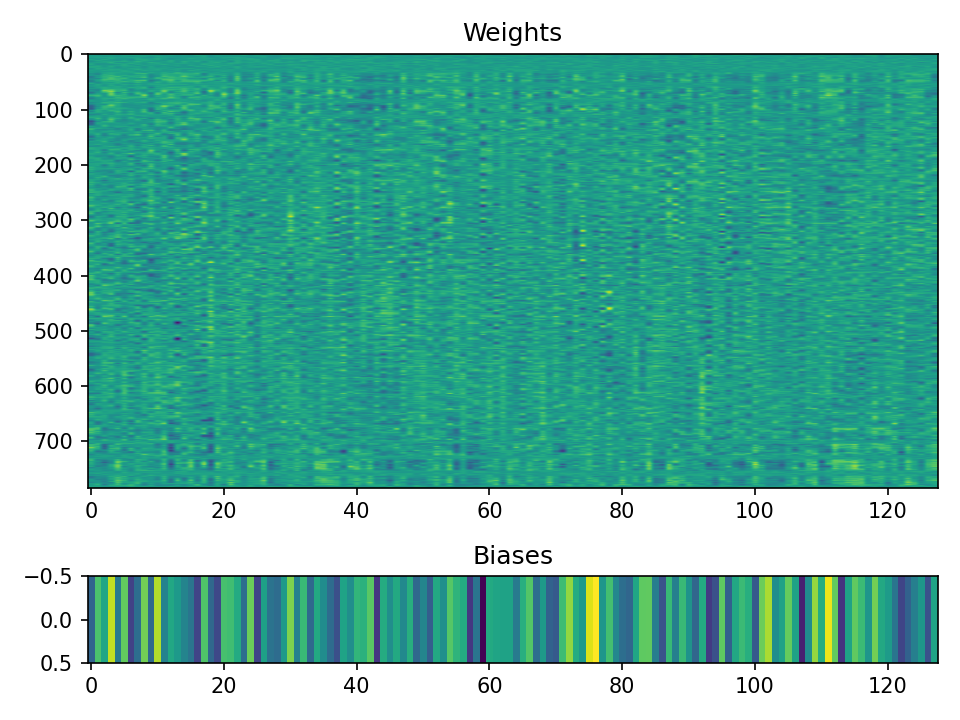
\includegraphics[width=0.8\linewidth]{figures/layer-1.png}
  \caption{First Layer Weights and Biases}
\end{figure}

\begin{figure}[H]
  \centering
  \pgfplotsset{/pgfplots/group/.cd,vertical sep=2.0cm}
  % This file was created with tikzplotlib v0.10.1.
\pgfplotsset{/pgfplots/group/.cd,vertical sep=1.6cm}
\begin{tikzpicture}
  \definecolor{darkgray176}{RGB}{176,176,176}
  \begin{groupplot}[group style={group size=1 by 2},width=0.7\textwidth]
    \nextgroupplot[
      tick align=outside,
      tick pos=left,
      title={Weights},
      x grid style={darkgray176},
      xmin=-0.5, xmax=9.5,
      xtick style={color=black},
      y dir=reverse,
      y grid style={darkgray176},
      ymin=-0.5, ymax=127.5,
      ytick style={color=black}
    ]
    \addplot graphics [includegraphics cmd=\pgfimage,xmin=-0.5, xmax=9.5, ymin=127.5, ymax=-0.5] {figures/generated/layer-2-000.png};

    \nextgroupplot[
      tick align=outside,
      tick pos=left,
      title={Biases},
      x grid style={darkgray176},
      xmin=-0.5, xmax=9.5,
      xtick style={color=black},
      y dir=reverse,
      y grid style={darkgray176},
      ymin=-0.5, ymax=0.5,
      ytick={0,1},
      ytick style={color=black},
      height=0.15\textwidth
    ]
    \addplot graphics [includegraphics cmd=\pgfimage,xmin=-0.5, xmax=9.5, ymin=0.5, ymax=-0.5] {figures/generated/layer-2-001.png};
  \end{groupplot}
\end{tikzpicture}

  % 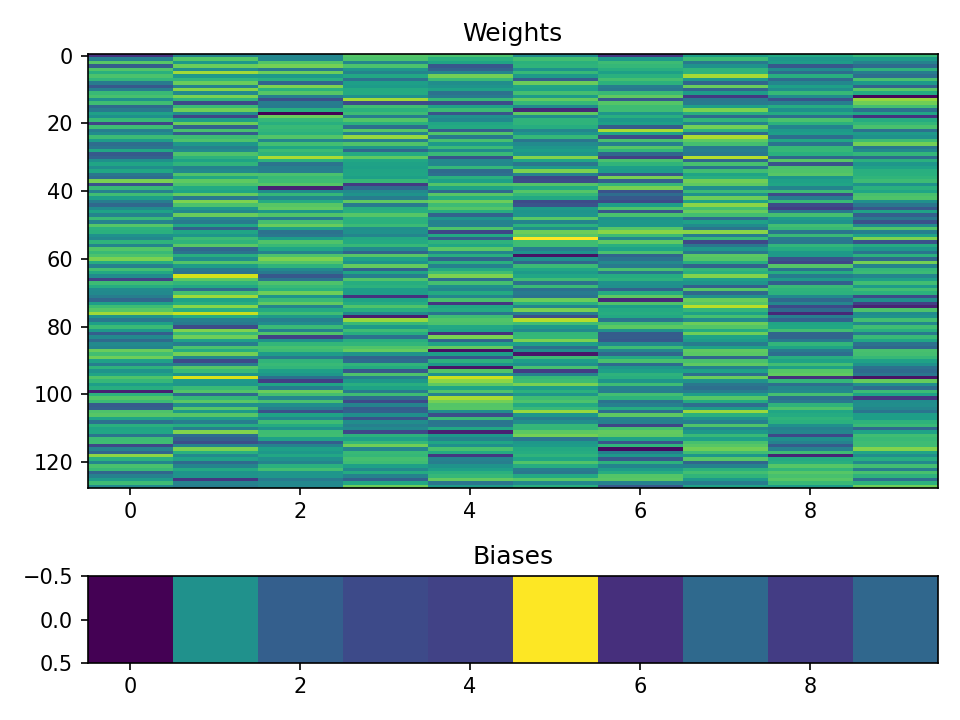
\includegraphics[width=0.8\linewidth]{figures/layer-2.png}
  \caption{Second Layer Weights and Biases}
\end{figure}
